
\documentclass{beamer} %ordinary
% \documentclass[handout]{beamer} % suppresses pauses into pdf handout

%\usepackage{hyperref}
%\usepackage{rotate}
%\usepackage{lscape}
%\usepackage{color}
%\usepackage{graphicx}
%\usepackage{amsmath}
%\usepackage{amsthm}
%\usepackage{epsfig}
%\usepackage{amssymb}
%\usepackage{rotating}
%\usepackage{psfrag}
\usepackage{amsfonts}


% \usetheme{default}
% \usetheme{Boadilla}
% \usetheme{Madrid}
% \usetheme{Montpellier}
 \usetheme{Warsaw}
% \usetheme{Copenhagen}
% \usetheme{Goettingen}
% \usetheme{Hannover}
% \usetheme{Berkeley}
% \usetheme{Malmoe}
% \usetheme{Pittsburgh}
% \usetheme[height=8mm]{Rochester}
% \usetheme{Singapore}
 
% \usecolortheme{crane}
 % \beamertemplatesolidbackgroundcolor{craneorange!25}
 \setbeamertemplate{navigation symbols}{}  %remove navigation icons
 \setbeamertemplate{headline}[default]


% comment command for multi-line comments: \comment{TEXT}
\newcommand{\comment}[1]{}


%%	Defined by Luis
\newcommand{\R}{ {\mathbb{R}} }
\newcommand{\1}{\mathbb{1}}
\newcommand{\argmin}{\operatornamewithlimits{argmin}}

%---------------------------------------------------------------------------------------------------------------------% 
\title[COSMOS 2016]{COSMOS 2016}
\subtitle{ The Difficulty of Science\\and\\Data Visualization} 

\author{Luis F. Campos}
 
\institute{Department of Statistics \\ Harvard University }

\date{July 22, 2016}
 %---------------------------------------------------------------------------------------------------------------------%
 


%%%%%%%%%%%%%%%%%%%%%%%%%%%%%%%%%%%%%%%%%%%%%
%%%%%%%%%%%%%%%%%%%%%%%%%%%%%%%%%%%%%%%%%%%%%
\begin{document}
%%%%%%%%%%%%%%%%%%%%%%%%%%%%%%%%%%%%%%%%%%%%%
%%%%%%%%%%%%%%%%%%%%%%%%%%%%%%%%%%%%%%%%%%%%%

 %---------------------------------------------------------------------------------------------------------------------%
\begin{frame}
	\titlepage	
\end{frame}
 %---------------------------------------------------------------------------------------------------------------------%
\begin{frame}{Outline}
  \tableofcontents
\end{frame}



\section{A crisis in science? (Reproducibility)}

\begin{frame}[t]\frametitle{A crisis in science? (Reproducibility)}
\vspace{3mm}
Reading (decreasing order of required-ness):\\
\vspace{3mm}
\begin{itemize}
	\item \href{http://www.nature.com/news/statisticians-issue-warning-over-misuse-of-p-values-1.19503}{\beamergotobutton{Nature: Statisticians issue warning over misuse of P values}}\\	
	\item \href{http://fivethirtyeight.com/features/science-isnt-broken/}{\beamergotobutton{FiveThirtyEight: Science Isn’t Broken}}\\	
	\item \href{http://www.nature.com/news/scientific-method-statistical-errors-1.14700}{\beamergotobutton{Nature: Scientific method: Statistical errors}}\\	
	\item \href{http://marginalrevolution.com/marginalrevolution/2016/07/results-free-review.html}{\beamergotobutton{Marginal Revolution: Results Free Review}}\\	
\end{itemize}

\end{frame}


\subsection{p-values, huh?}

\begin{frame}[t]\frametitle{p-value: what it is and what it is not}
	An example:\\
	\begin{itemize}
		\item You want to see if a new drug works \pause
		\item Give it to 50 people, see that it works for 49 people. \pause
		\item If we assume that the drug does not work, this is very unlikely. \pause
		\item If instead it worked for only 10 people. \pause
		\item Assuming that the drug does not work, 10 is fairly likely. \pause
	\end{itemize}
	\vspace{3mm}
	What it is:\\
	{\bf{p-value}}: If a certain hypothesis (drug doesn't work) is true, {\emph{and all other assumptions made are valid}}, what is are the odds we see the results we saw. \pause
	\begin{itemize}
		\item An implementation of the scientific process
	\end{itemize}

\end{frame}

\begin{frame}[t]\frametitle{p-value: what it is and what it is not}

{\bf{What it is}}:\\
	{\bf{p-value}}: If a certain hypothesis (drug doesn't work) is true, {\emph{and all other assumptions made are valid}}, what is are the odds we see the results we saw.\\
\vspace{3mm}
\pause
{\bf{What it is not}}:
\begin{itemize}
	\item The probability of a hypothesis being true \pause
	\item A replacement for science (science is hard) \pause
	\item A justification for publication \pause
\end{itemize}

\href{http://www.nature.com/news/statisticians-issue-warning-over-misuse-of-p-values-1.19503}{\beamergotobutton{Nature: Statisticians issue warning over misuse of P values}}\\	
\end{frame}

\subsection{Publication Bias}

\begin{frame}[t]\frametitle{Publication Bias}

What is publication bias?
\vspace{3mm}
\begin{itemize}
	\item Say researchers test 100 hypotheses
	\begin{itemize}
		\item[] e.g. test to see if a new drug/treatment works
	\end{itemize}
	\item About $5\%$ will be ``statistically significant'' even is none of them actually work
	\item These are usually the (only) ones we see in publication.
\end{itemize}
\pause
What's the issue? 
\pause
\begin{itemize}
	\item Because publications mean a lot to scientists, they are motivated to ``hack'' their studies to significance
	\pause
	\begin{itemize}
		\item p-Hacking
		\item (Sometimes happens unintentionally as well)
	\end{itemize}
\end{itemize}

\href{http://marginalrevolution.com/marginalrevolution/2016/07/results-free-review.html}
{\beamergotobutton{A potential solution to publication bias}}\\	
\end{frame}


\subsection{p-Hacking}

\begin{frame}[t]\frametitle{A bit about p-Hacking}

Science, what's the issue?  \pause
\begin{itemize}
	\item Hard 
	\item Expensive 
	\item Time Consuming \pause
	\item The best tool we have for reaching the truth 
\end{itemize}
\vspace{3mm}
{\bf{Why is it so hard to get a rigorous result?!}}
\vspace{3mm}

\href{http://fivethirtyeight.com/features/science-isnt-broken/}
{\beamergotobutton{Let's do an exercise}}\\	
\end{frame}


\begin{frame}[t]\frametitle{A p-Hacking Example}

If you select 
\begin{itemize}
	\item Representatives and Senators to calculate ``in office''
	\item GDP and stock-prices to measure a ``better economy''
\end{itemize}
\vspace{3mm}
You'll find that when there are more Democrats in power, the economy is ``significantly'' better
\vspace{3mm}

If you select 
\begin{itemize}
	\item Presidents and Governors to calculate ``in office''
	\item employment and inflation to measure a ``better economy''
\end{itemize}
\vspace{3mm}
You'll find that when there are more Republicans in power, the economy is ``significantly'' better

\end{frame}



\begin{frame}[t]\frametitle{A p-Hacking Example}

\vspace{5mm}
\begin{itemize}
	\item This shouldn't be interpreted as ``Science is unreliable and fickle''.
	\item Instead, ``Science is harder than we give it credit for''.
\end{itemize}
\vspace{5mm}

Hopefully going through this exercise gave you some things to look for in academic papers:
\begin{itemize}
	\item Did they describe their data transparently?
	\item Did they describe their analysis in detail?
	\item Did they justify the choices they made? (e.g. why these variables?)
\end{itemize}


\end{frame}



\begin{frame}[t]\frametitle{Some possible Solutions to this}

Maybe we should ``encourage'' p-hacking?
\begin{itemize}
	\item Of course, these decisions should be transparent
	\item Some call this pseudo-science
	\item This isn't science but that doesn't mean it's not meaningful 
\end{itemize}
\vspace{3mm}
\pause
Maybe we should ``encourage'' retractions?
\begin{itemize}
	\item Number of retractions are going up, but not fast enough
	\item Replication studies should be encouraged
	\item Should be part of the publishing/scientific process
\end{itemize}

\href{http://fivethirtyeight.com/features/science-isnt-broken/}
{\beamergotobutton{Reading Assignment 2}}\\	
\end{frame}



\subsection{Some Hope for the Future}

\begin{frame}[t]\frametitle{Some Hope for the Future}

\begin{itemize}
	\item ``People want to prove something, and a negative result doesn’t satisfy that craving'' \pause
	\item ``Science is low-yield. Most experiments fail'' but that's okay \pause
	\item ``Once an idea becomes fixed, it’s difficult to remove from the conventional wisdom'' \pause
	\item ``Science is not a magic wand that turns everything it touches to truth'' \pause
	\item ``Science isn’t broken, it’s just more difficult than most of us realize'' \pause
\end{itemize}

\vspace{3mm}
 % {\bf{\Large{Thank you!}}}

\end{frame}





% - - - - - - - - - - - - - - - - - - - - - - - - - - - - - - - -%
%				Introduction
% - - - - - - - - - - - - - - - - - - - - - - - - - - - - - - - -%


\section[Data Visualization]{Data Visualization}

\subsection[Why is visualizing data important?]{Why is visualizing data important?}

\begin{frame}[t]\frametitle{Visualizing data}
\begin{center}
{\bf{What are visualizations?}}
\vspace{2 mm}
\begin{itemize}
	\item Graphical representations of information.
	\item Tools to help us communicate and learn.
	\item Pretty pictures/interfaces.
\end{itemize}
\end{center}
\vspace{5 mm}
\pause

\begin{center}
{\bf{Why is visualizing data important?}}
\vspace{2 mm}

\begin{itemize}
	\item Convey a large amount of information.
	\item Helps tell a story.
	\item Draws in the reader.
\end{itemize}
\end{center}

\end{frame}

% - - - - - - - - - - - - - - - - - - - - - - - - - - - - - - - -%
%					Facebook example - visualization
% - - - - - - - - - - - - - - - - - - - - - - - - - - - - - - - -%

\subsection[Visualizing data - Facebook]{Facebook example}

\begin{frame}[t]\frametitle{Facebook example}
	\begin{center}
		
\includegraphics[scale = 0.3]{./visualization/facebook_logo.jpg}
	\end{center}
\end{frame}
\begin{frame}[t]\frametitle{Facebook - 2010}
	\begin{center}
		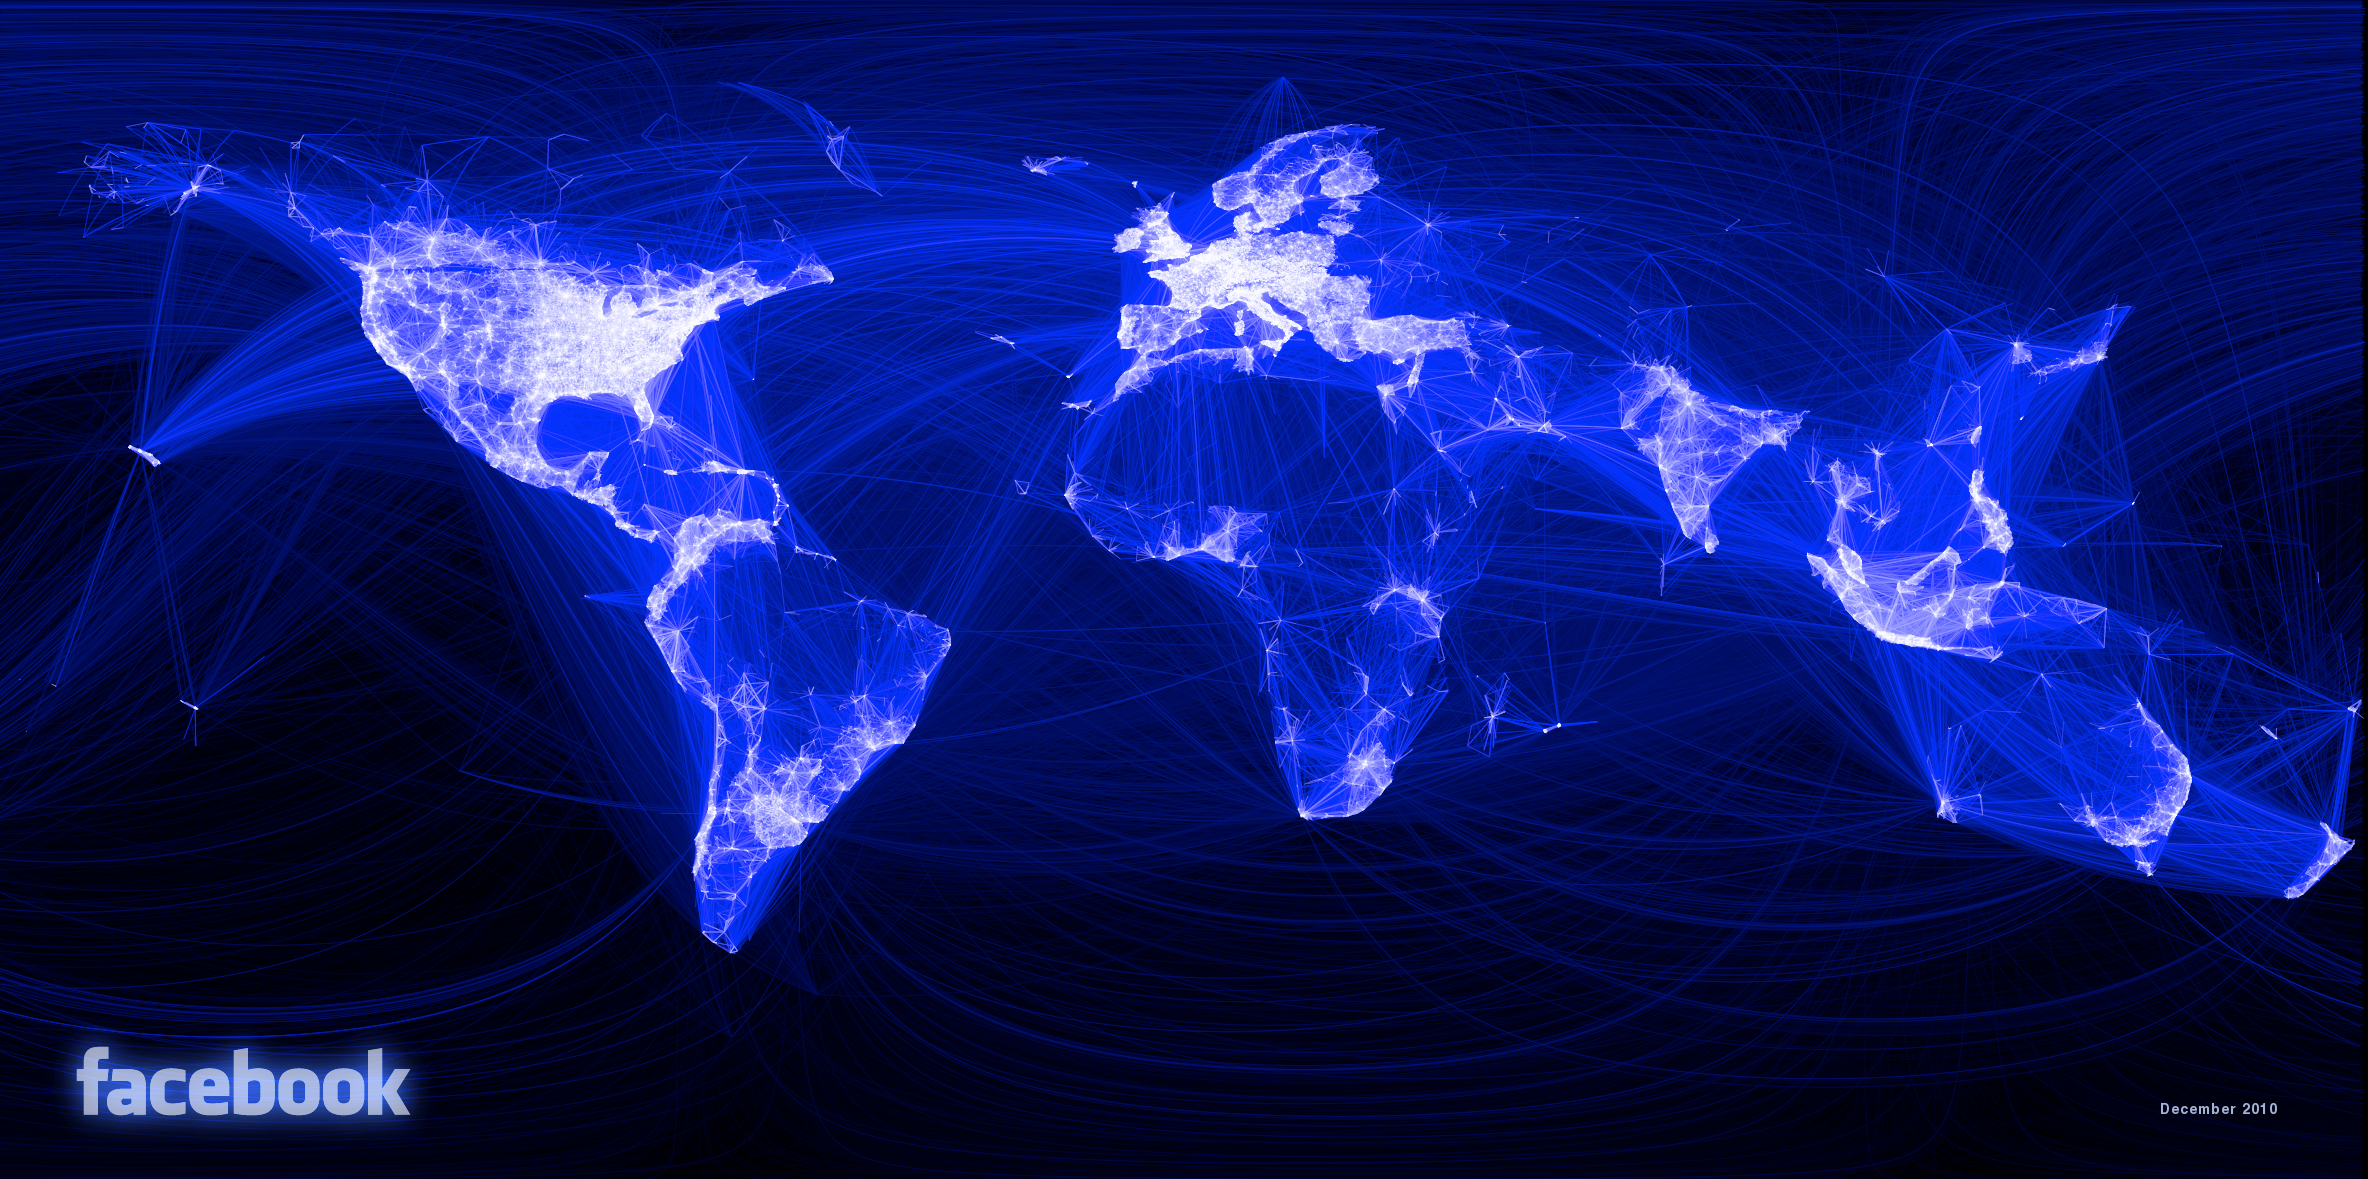
\includegraphics[scale = 0.13]{./visualization/facebook.jpg}
	\end{center}
	\begin{itemize}
		\item The line intensity from blue to white represents the number of connections between cities. 
	\end{itemize}
\end{frame}
\begin{frame}[t]\frametitle{Facebook - 2013}
	\begin{center}
		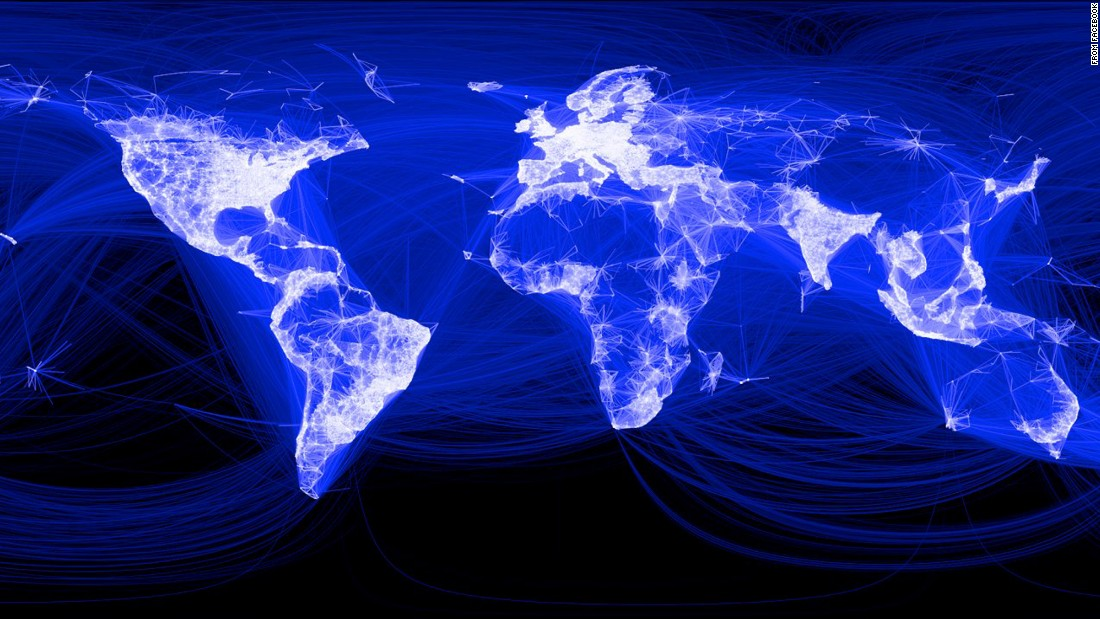
\includegraphics[scale = 0.275]{./visualization/facebook2013.jpg}
	\end{center}
	\begin{itemize}
		\item Most recent version I could find.
	\end{itemize}
\end{frame}

\begin{frame}[t]\frametitle{Facebook example}
	\begin{center}
		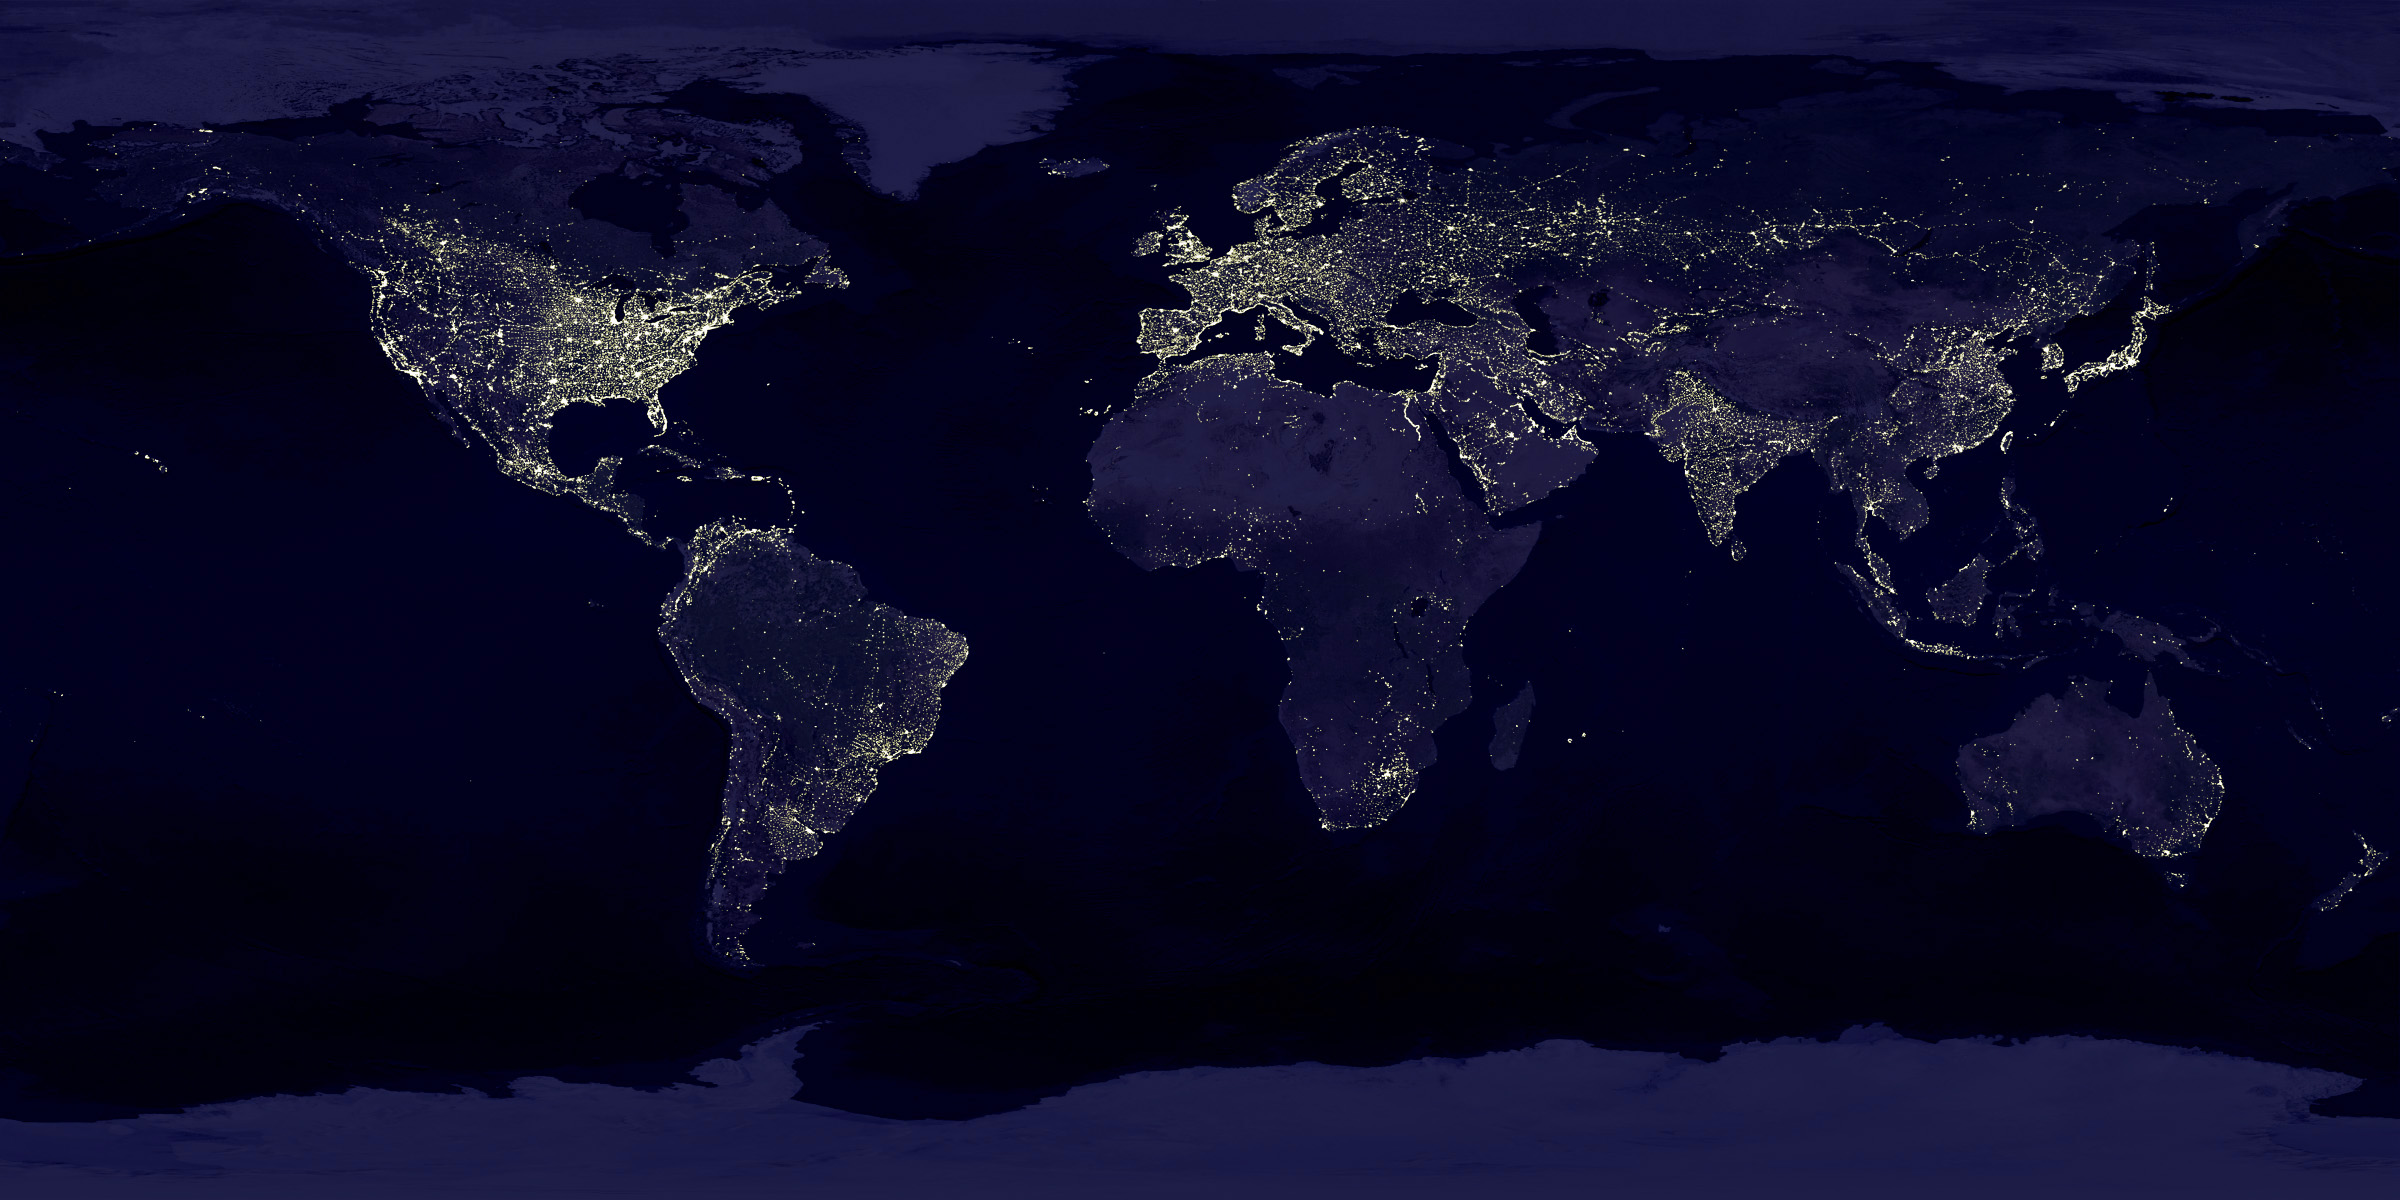
\includegraphics[scale = 0.18]{./visualization/earth_night.jpg}
	\end{center}
\end{frame}

\begin{frame}[t]\frametitle{Facebook example}
\begin{center}
		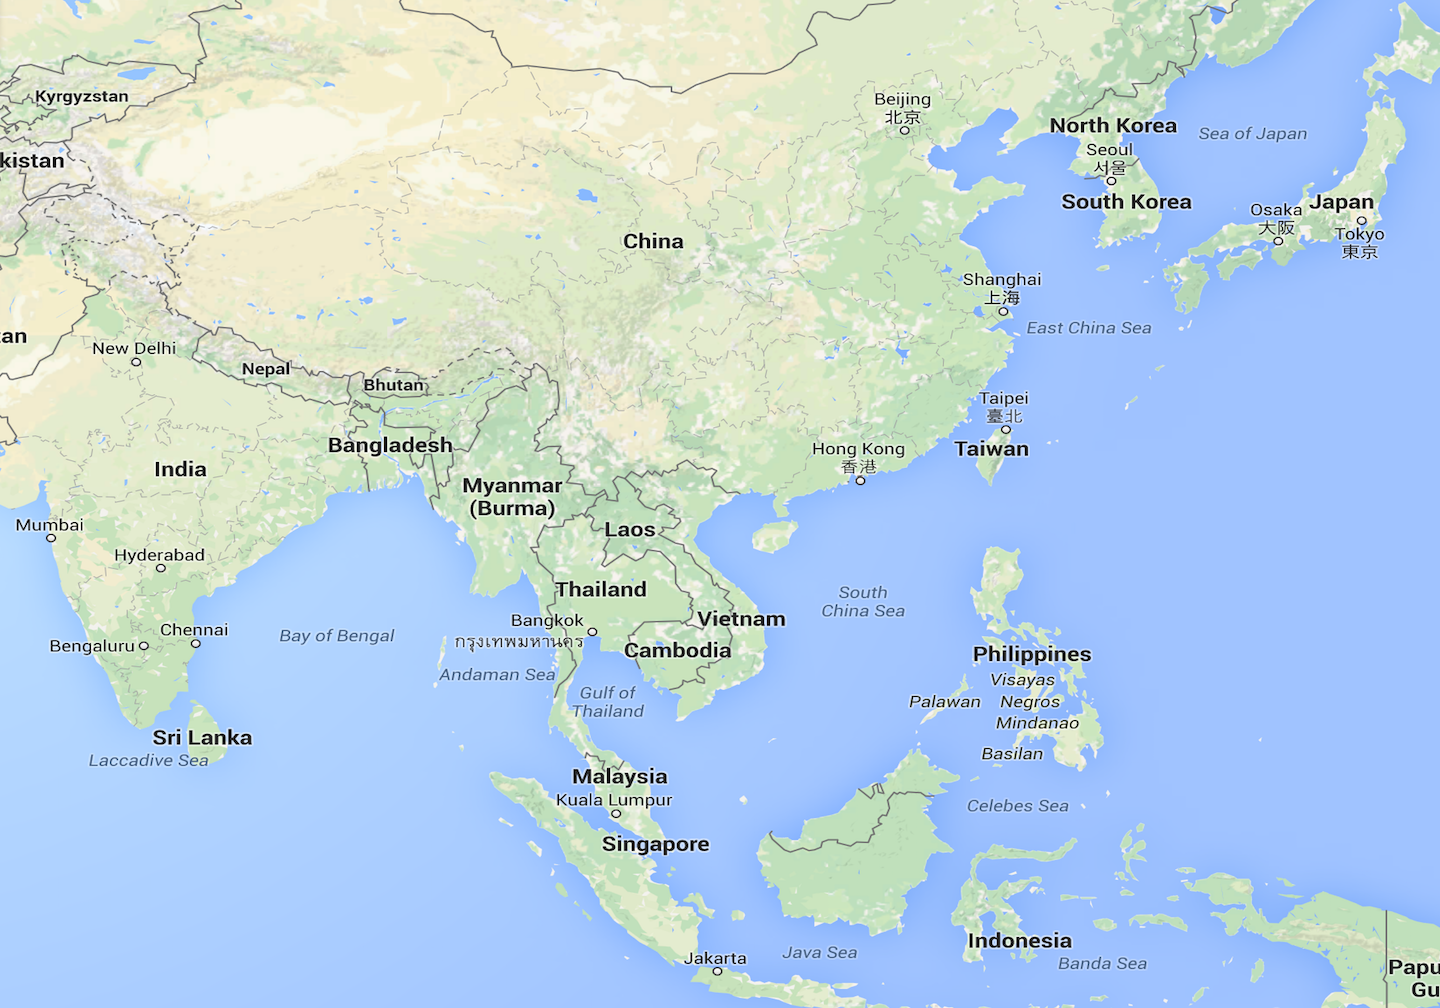
\includegraphics[scale = 0.22]{./visualization/SEAsia_map.png}
		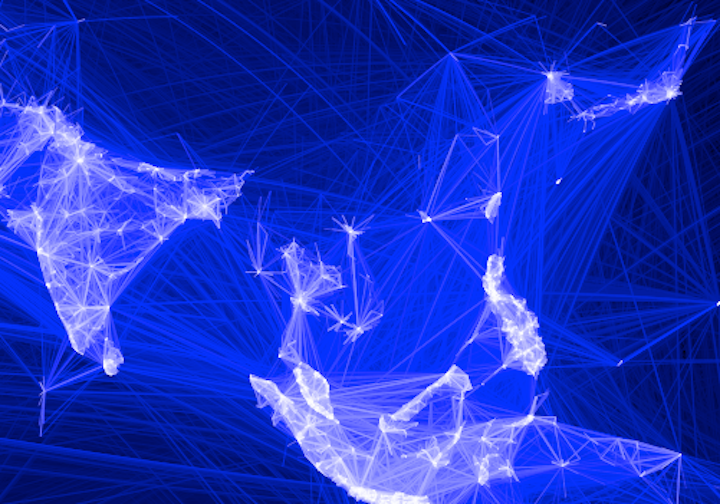
\includegraphics[scale = 0.22]{./visualization/SEAsia_fb.png}
	\end{center}
	Do you notice anything interesting? Try finding the countries.
	\pause
	\begin{itemize}
		\item India, Japan, Malaysia, the Philippines are all fully connected
		\item China is not prominent at all... \pause except for Hong Kong.
	\end{itemize}
\end{frame}



\begin{frame}[t]\frametitle{Facebook example}
	\begin{center}
		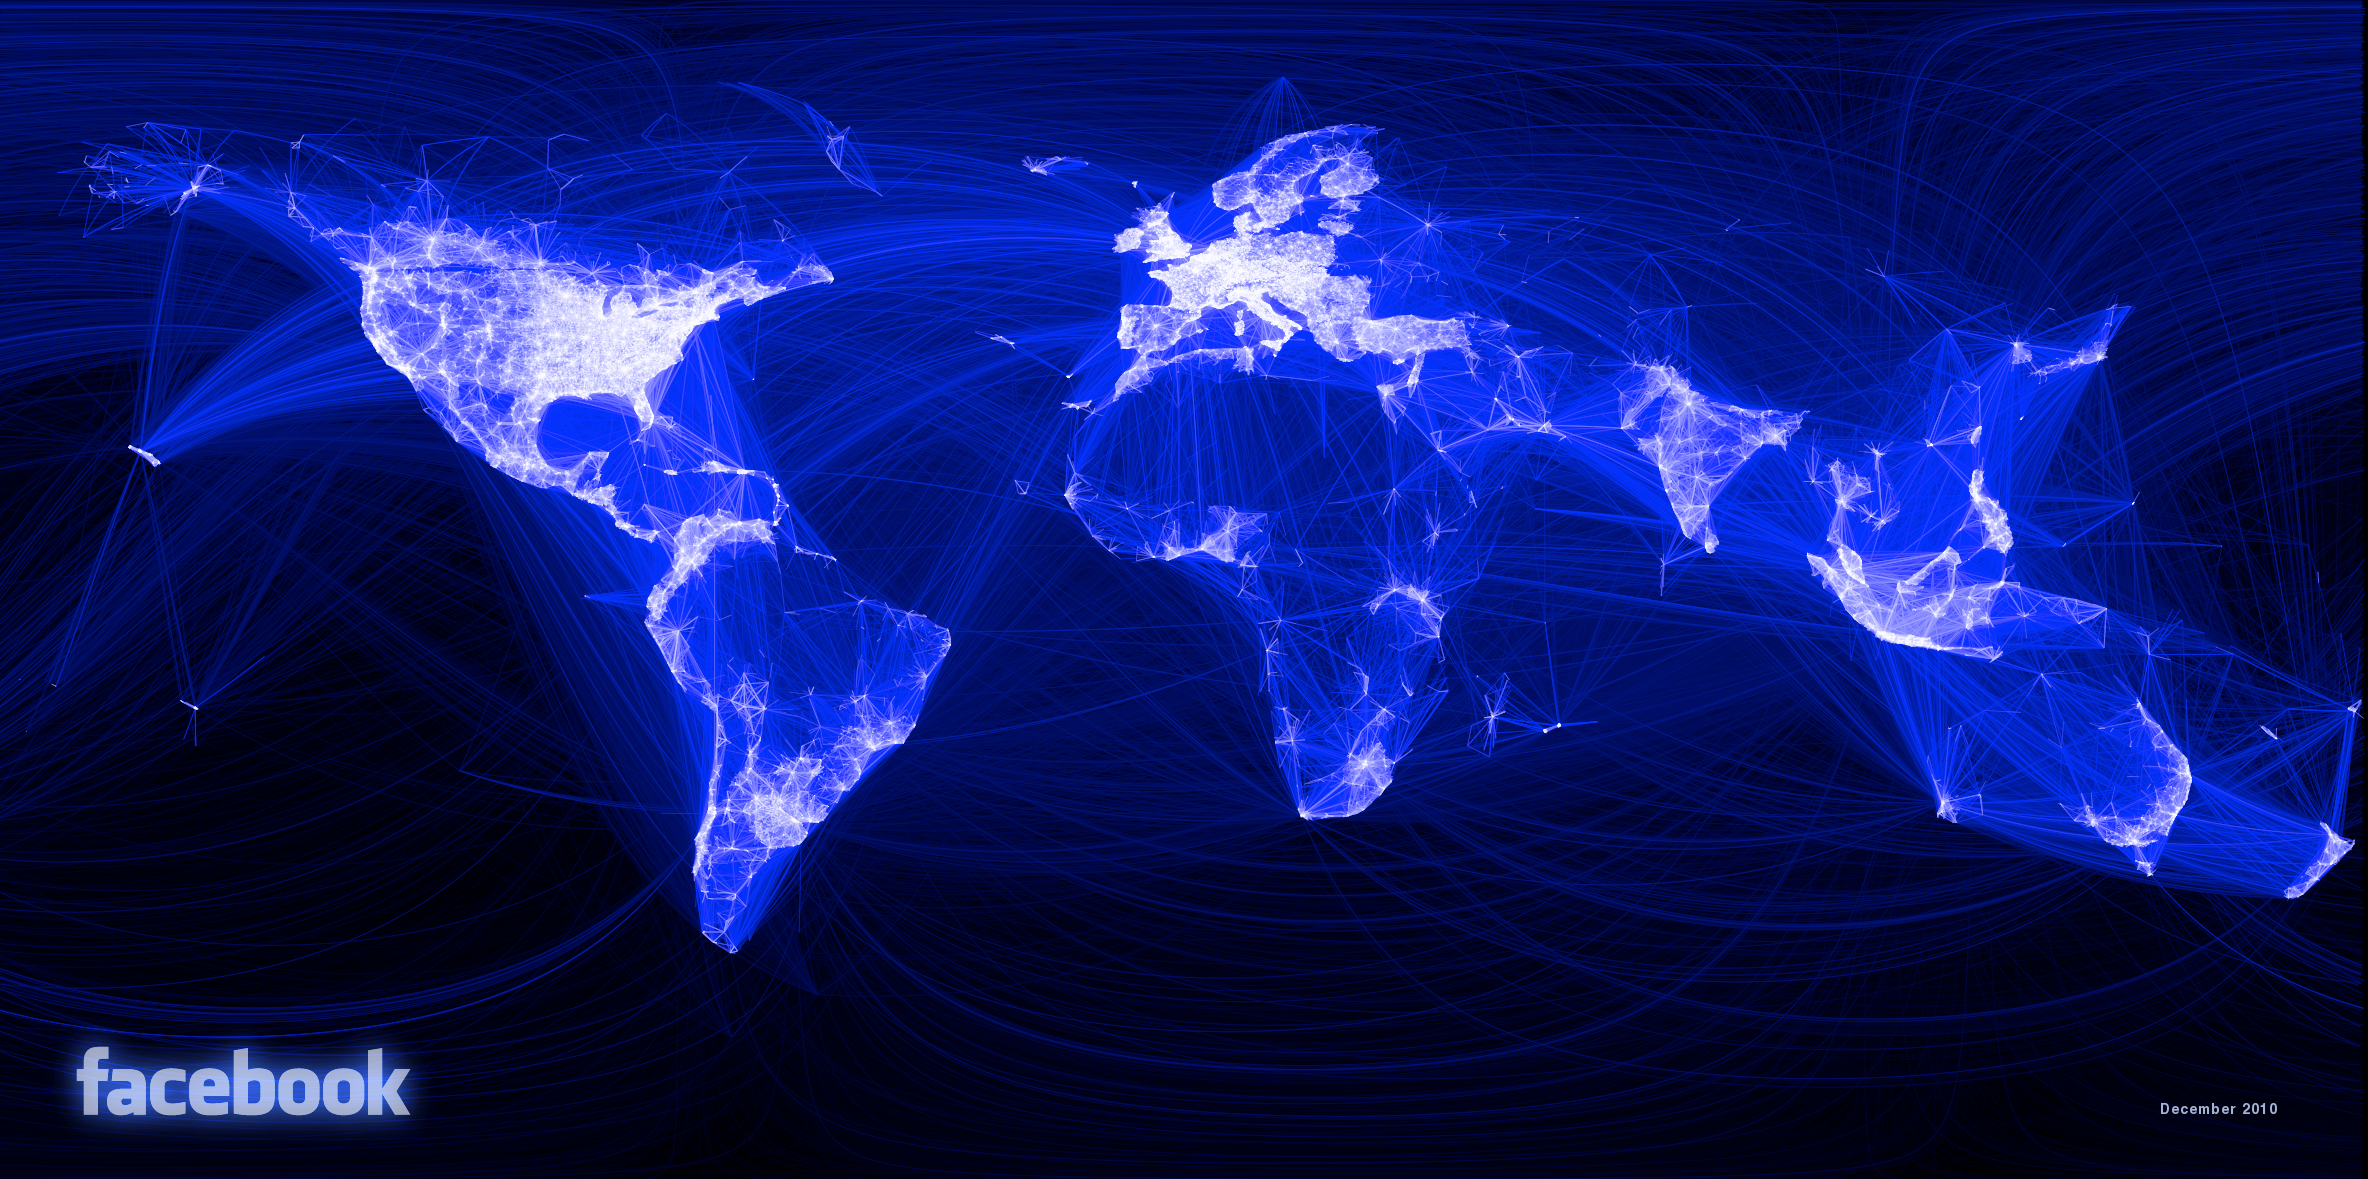
\includegraphics[scale = 0.05]{./visualization/facebook.jpg}
	\end{center}
    
    \begin{itemize}
    	\item Recall: the line intensity represents the number of connections between cities -- that's all. 
    	\item We found geography.
    	\item When data is organized in a simple and intuitive way you can explore and find other interesting things.
    \end{itemize}
\end{frame}


% % % % % % % % % % % % % % % % % % % % % % % 
\comment{
% % % % % % % % % % % % % % % % % % % % % % % 

				% - - - - - - - - - - - - - - - - - - - - - - - - - - - - - - - -%
				%					Unemployment example - visualization
				% - - - - - - - - - - - - - - - - - - - - - - - - - - - - - - - -%

				\subsection[Visualizing data - Unemployment]{Unemployment example}

				\begin{frame}[t]\frametitle{US state-level unemployment rate}
				Let's look at some state-level data

				% - - - - - - - - - - - - - - - - - - - - - - - - - - - - - - - -%
				%	This is how you create a link
				% - - - - - - - - - - - - - - - - - - - - - - - - - - - - - - - -%

				\href{http://www.bls.gov/eag/eag.ca.htm}{\beamergotobutton{Bureau of Labor Statistics: California Unemployment}}

				\href{http://www.bls.gov/bls/newsrels.htm}{\beamergotobutton{Bureau of Labor Statistics: Other Tables}}


				You can probably see how looking at the data like this will make it hard to learn much.\\
				\begin{itemize}
					\item How about a map?
				\end{itemize}


				\end{frame}

				\begin{frame}[t]\frametitle{US state-level unemployment rate}
				\includegraphics[scale = 0.52, page = 1]{./visualization/monthly_unemployment_byState.pdf}
				\end{frame}

				%%%%%%%%%%%
				% \comment{
				%%%%%%%%%%%

				\begin{frame}[t]\frametitle{US state-level unemployment rate}
				\includegraphics[scale = 0.52, page = 3]{./visualization/monthly_unemployment_byState.pdf}
				\end{frame}

				\begin{frame}[t]\frametitle{US state-level unemployment rate}
				\includegraphics[scale = 0.52, page = 4]{./visualization/monthly_unemployment_byState.pdf}
				\end{frame}

				\begin{frame}[t]\frametitle{US state-level unemployment rate}
				\includegraphics[scale = 0.52, page = 5]{./visualization/monthly_unemployment_byState.pdf}
				\end{frame}

				\begin{frame}[t]\frametitle{US state-level unemployment rate}
				\includegraphics[scale = 0.52, page = 6]{./visualization/monthly_unemployment_byState.pdf}
				\end{frame}

				\begin{frame}[t]\frametitle{US state-level unemployment rate}
				\includegraphics[scale = 0.52, page = 7]{./visualization/monthly_unemployment_byState.pdf}
				\end{frame}

				\begin{frame}[t]\frametitle{US state-level unemployment rate}
				\includegraphics[scale = 0.52, page = 8]{./visualization/monthly_unemployment_byState.pdf}
				\end{frame}


				\begin{frame}[t]\frametitle{US state-level unemployment rate}
				\includegraphics[scale = 0.52, page = 10]{./visualization/monthly_unemployment_byState.pdf}
				\end{frame}

				\begin{frame}[t]\frametitle{US state-level unemployment rate}
				\includegraphics[scale = 0.52, page = 11]{./visualization/monthly_unemployment_byState.pdf}
				\end{frame}

				\begin{frame}[t]\frametitle{US state-level unemployment rate}
				\includegraphics[scale = 0.52, page = 12]{./visualization/monthly_unemployment_byState.pdf}
				\end{frame}

				\begin{frame}[t]\frametitle{US state-level unemployment rate}
				\includegraphics[scale = 0.52, page = 13]{./visualization/monthly_unemployment_byState.pdf}
				\end{frame}

				\begin{frame}[t]\frametitle{US state-level unemployment rate}
				\includegraphics[scale = 0.52, page = 14]{./visualization/monthly_unemployment_byState.pdf}
				\end{frame}

				\begin{frame}[t]\frametitle{US state-level unemployment rate}
				\includegraphics[scale = 0.52, page = 15]{./visualization/monthly_unemployment_byState.pdf}
				\end{frame}

				\begin{frame}[t]\frametitle{US state-level unemployment rate}
				\includegraphics[scale = 0.52, page = 16]{./visualization/monthly_unemployment_byState.pdf}
				\end{frame}

				\begin{frame}[t]\frametitle{US state-level unemployment rate}
				\includegraphics[scale = 0.52, page = 17]{./visualization/monthly_unemployment_byState.pdf}
				\end{frame}

				\begin{frame}[t]\frametitle{US state-level unemployment rate}
				\includegraphics[scale = 0.52, page = 18]{./visualization/monthly_unemployment_byState.pdf}
				\end{frame}

				\begin{frame}[t]\frametitle{US state-level unemployment rate}
				\includegraphics[scale = 0.52, page = 19]{./visualization/monthly_unemployment_byState.pdf}
				\end{frame}

				\begin{frame}[t]\frametitle{US state-level unemployment rate}
				\includegraphics[scale = 0.52, page = 20]{./visualization/monthly_unemployment_byState.pdf}
				\end{frame}

				\begin{frame}[t]\frametitle{US state-level unemployment rate}
				\includegraphics[scale = 0.52, page = 21]{./visualization/monthly_unemployment_byState.pdf}
				\end{frame}

				\begin{frame}[t]\frametitle{US state-level unemployment rate}
				\includegraphics[scale = 0.52, page = 22]{./visualization/monthly_unemployment_byState.pdf}
				\end{frame}

				%%%%%%%%%%%
				% }
				%%%%%%%%%%%


				\begin{frame}[t]\frametitle{US state-level unemployment rate}
				\includegraphics[scale = 0.52, page = 23]{./visualization/monthly_unemployment_byState.pdf}
				\end{frame}

				\begin{frame}[t]\frametitle{What did we learn?}
					\begin{itemize}
						\item Unemployment rates seem to be geographically related
						\item In the middle of 2008 we were increasing by about 0.2\% per month
						\item By Early 2009, we were increasing by about 0.5\% per month
						\item In the period we investigated the unemployment rate nearly doubled.
					\end{itemize}
					This just leads to more questions:
					\begin{itemize}
						\item Can these increase rates can be visualized much simpler?
						\item How do the rates look through time for different states?
						\item What about historical trends?
					\end{itemize}

				\end{frame}


				\begin{frame}[t]\frametitle{US state-level unemployment rate}
				But this might be easier to see by seeing the raw unemployment rate through time. 
				\\
				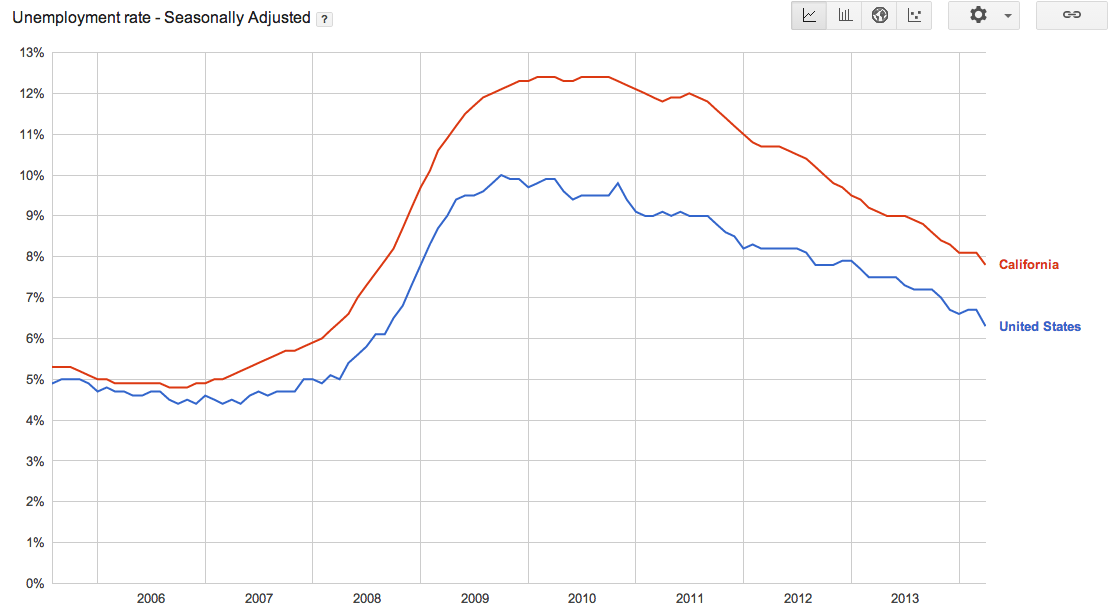
\includegraphics[scale = 0.29]{./visualization/unemployment_trend.png}
				\end{frame}


				\begin{frame}[t]\frametitle{US state-level unemployment rate}
				What about historical trends?
				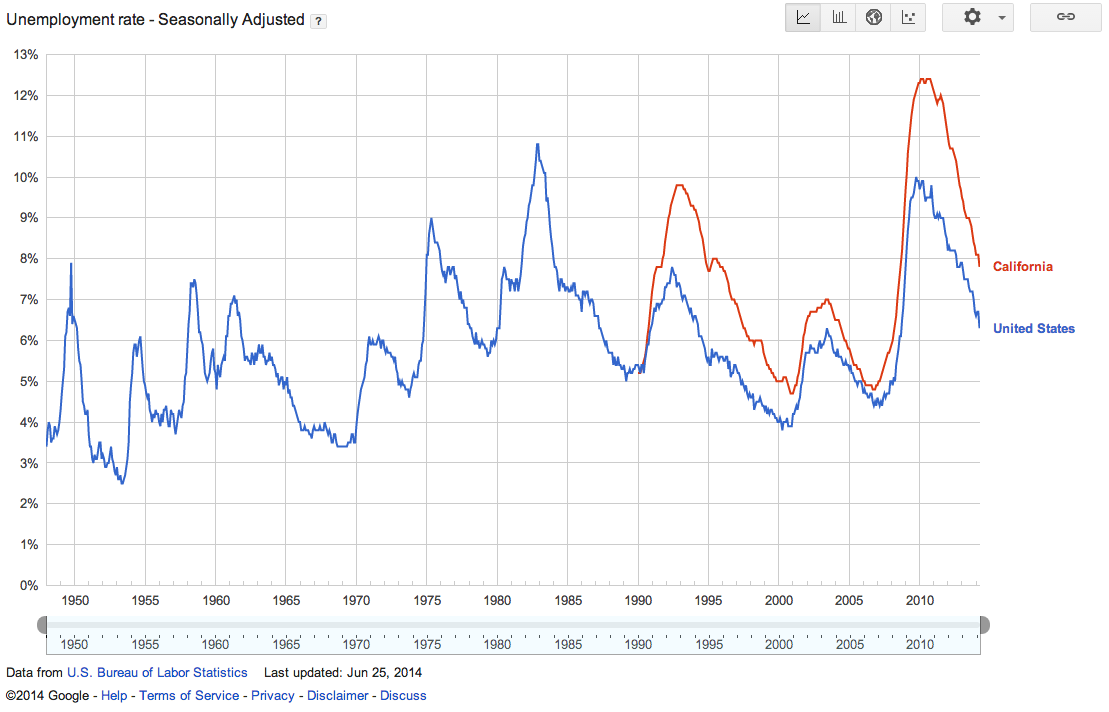
\includegraphics[scale = 0.29]{./visualization/unemployment_rate_historical.png}
				\end{frame}


				\begin{frame}[t]\frametitle{Visualization helps tell a story}
				\href{https://www.google.com/publicdata/explore?ds=z1ebjpgk2654c1_&met_y=unemployment_rate}{\beamergotobutton{Google trends}}\\
				Unemployment in the U.S:
				\begin{itemize}
					\item Unemployment rates seem to be geographically related
					\item in 2008 we had a dramatic increase in unemployment
					\item there has been a steady decrease since 2009, but we're still 3\% higher than in 2006
					\item we saw a similar trend during the recession of the early 80s
				\end{itemize}
				\end{frame}

% % % % % % % % % % % % % % % % % % % % % % % 
}
% % % % % % % % % % % % % % % % % % % % % % % 



% - - - - - - - - - - - - - - - - - - - - - - - - - - - - - - - -%
%					Vernacular example - visualization
% - - - - - - - - - - - - - - - - - - - - - - - - - - - - - - - -%

\subsection[Visualizing data - vernacular]{Vernacular example}
\begin{frame}[t]\frametitle{Vernacular across the U.S.}
{\bf{What do you call a sweetened carbonated beverage?}}
\begin{itemize}
	\item Soda
	\item Pop
	\item Coke
\end{itemize}

\end{frame}

\begin{frame}[t]\frametitle{Vernacular across the U.S.}
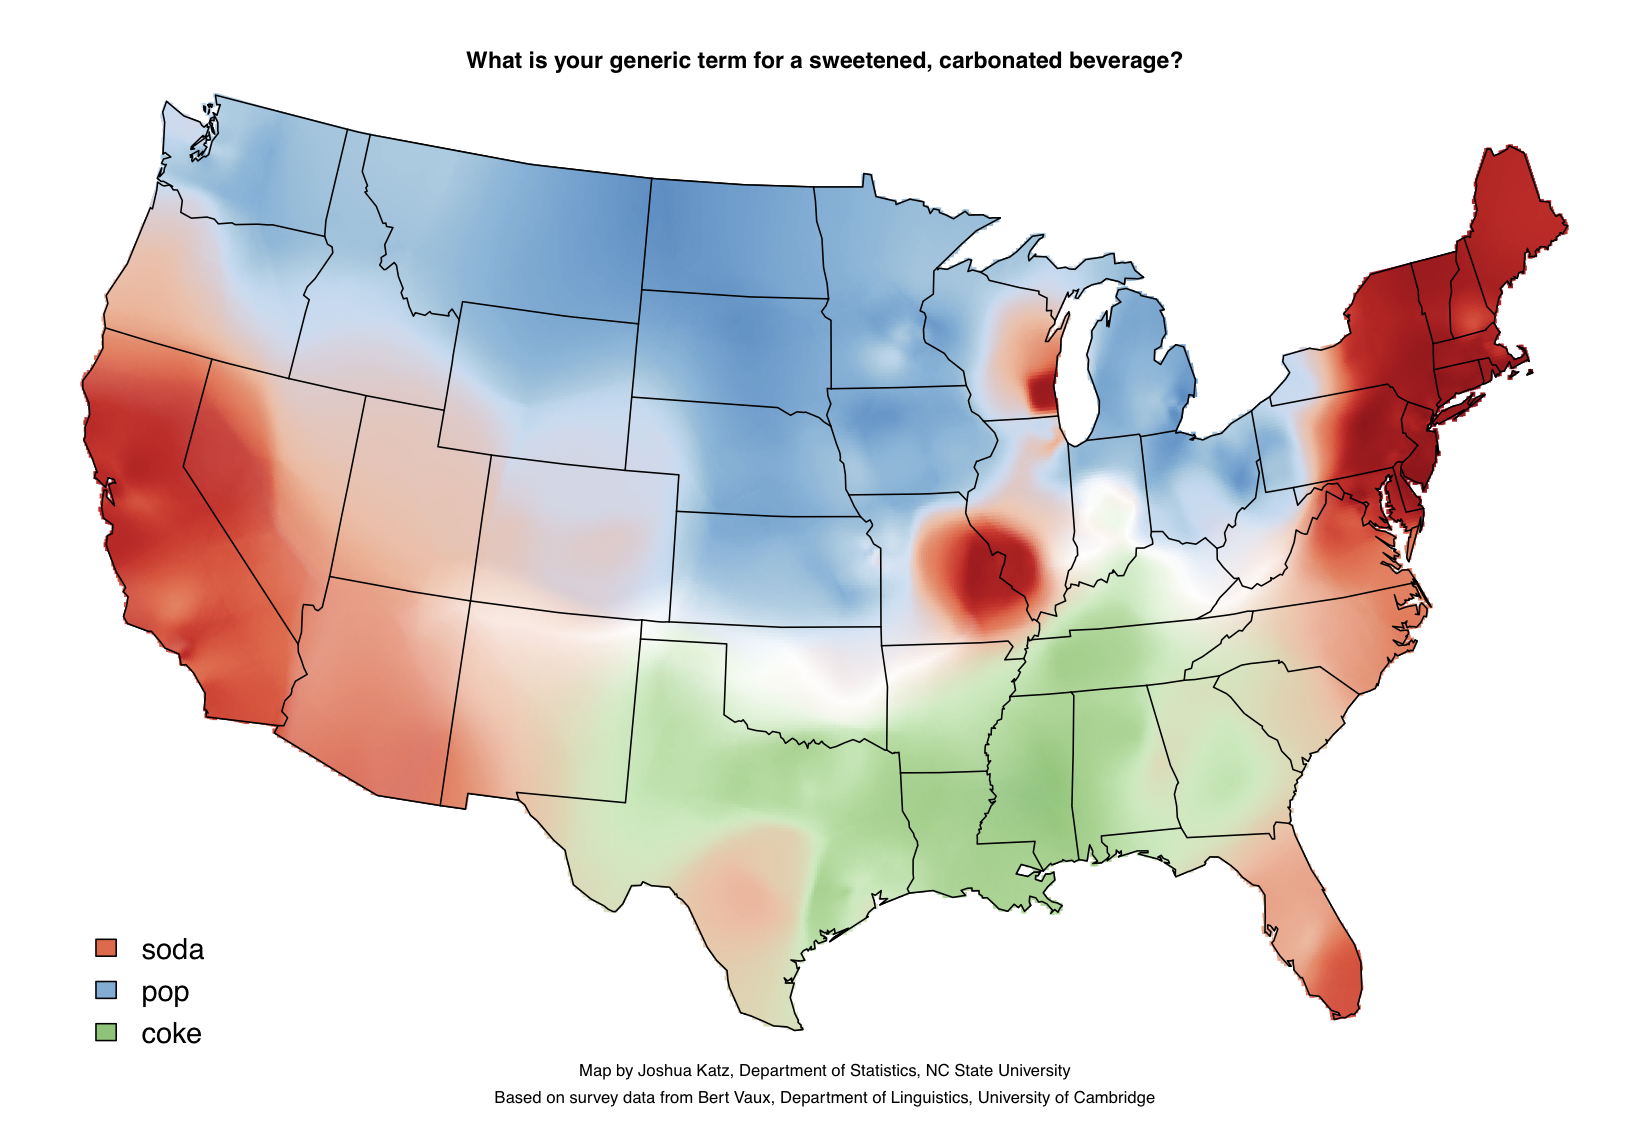
\includegraphics[scale = 0.4]{./visualization/sodapopcoke.png}
\end{frame}

\begin{frame}[t]\frametitle{Vernacular across the U.S.}
We can ask other questions that might have different answers depending on where you're from
\begin{itemize}
	\item  what do you call the long sandwich that contains cold cuts, lettuce, and so on?
	\begin{itemize}
		\item Sub, hoagie, Italian sandwich, etc.
	\end{itemize}
	\item how do you pronounce ``caramel''?
	\begin{itemize}
		\item car-ml, carra-mel, either
	\end{itemize}	
	\item what word(s) do you use to address a group of two or more people?
	\begin{itemize}
		\item you guys, you, y'all, you all
	\end{itemize}	
	\item[]
\end{itemize}
\href{http://www4.uwm.edu/FLL/linguistics/dialect/maps.html}{\beamergotobutton{More Questions}}

\end{frame}


\begin{frame}[t]\frametitle{Vernacular across the U.S.}
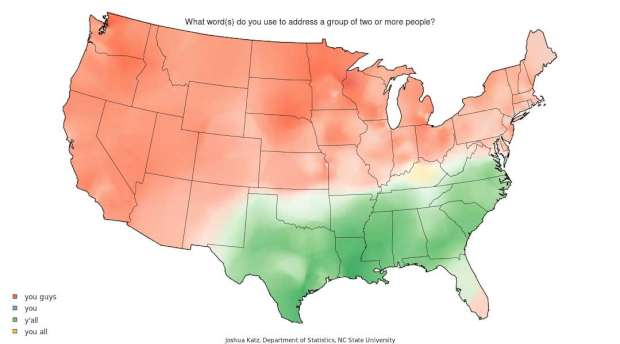
\includegraphics[scale = 0.4]{./visualization/you_all.jpg}
\end{frame}

\begin{frame}[t]\frametitle{Vernacular across the U.S.}
What are some natural questions?
\begin{itemize}
	\item If we have how people in a particular area respond to a long list of questions, can we use this to see what cities are similar to each other?
	\item This might be important if you're traveling!
	\item It's also just fun. 
\end{itemize}
\end{frame}


\begin{frame}[t]\frametitle{Vernacular example - What does it mean to be similar?}
	Questions
	\begin{enumerate}
\item what do you call a sweetened carbonated beverage? 
	 	\begin{itemize}
	 		\item soda = 0 $\qquad$ pop = 1
	 	\end{itemize}
	 	\item what do you call the long sandwich that contains cold cuts, lettuce, and so on?
	 	\begin{itemize}
	 		\item sub = 0 $\qquad$ hoagie = 1
	 	\end{itemize}
	 	\item how do you pronounce ``caramel''? 
	 	\begin{itemize}
	 		\item car-ml = 0 $\qquad$ carra-mel = 1
	 	\end{itemize}
	 	\item what word(s) do you use to address a group of two or more people?
	 	\begin{itemize}
	 		\item you guys = 0 $\qquad$ y'all = 1
	 	\end{itemize}
	 \end{enumerate} 
\end{frame}


\begin{frame}[t]{Vernacular example - What does it mean to be similar?}
Person 1: soda, sub, carra-mel, you guys\\
Person 2: soda, sub, car-ml, you guys\\
Person 3: pop, hoagie, carra-mel, y'all\\
\vspace{5 mm}
How does this translate to numbers?
\begin{enumerate}
	\item 0, 0, 1, 0
	\item 0, 0, 0, 0
	\item 1, 1, 1, 1
\end{enumerate}

\vspace{3mm}
\pause
Who is the most similar in their responses?\\
Who is most different in their responses?\\

\vspace{3mm}
\pause
Most Similar:  ($1 <-> 2$)\\
Most Different:  ($2 <-> 3$)\\

\end{frame}

\begin{frame}\frametitle{Vernacular example - What does it mean to be similar?}
We can use the distance between these two people to assess similarity
\begin{align*}
d(p_1, p_2) &= |0 - 0| + |0 - 0| + |1 - 0| + |0 - 0| = 1\\
d(p_2, p_3) &= |0 - 1| + |0 - 1| + |0 - 1| + |0 - 1| = 4\\
d(p_1, p_3) &= |0 - 1| + |0 - 1| + |1 - 1| + |0 - 1| = 3 \
% d(p_1, p_2) &= \sqrt{(0 - 0)^2 + (0 - 0)^2 + (1 - 0)^2 + (0 - 0)^2} = \sqrt{1} = 1\\
% d(p_2, p_3) &= \sqrt{(0 - 1)^2 + (0 - 1)^2 + (0 - 1)^2 + (0 - 1)^2} = \sqrt{4} = 2\\
% d(p_1, p_3) &= \sqrt{(0 - 1)^2 + (0 - 1)^2 + (1 - 1)^2 + (0 - 1)^2} = \sqrt{3} \approx 1.73
\end{align*}

This is called the ``Manhattan'' distance. Can anyone guess why?

\vspace{3 mm}
\begin{itemize}
	\item If we do this for all the people in the survey, we can see which people are similar!
	\item If we want to find out what regions are similar to a particular person ($p_1$), we can look at all $d(p_1, p_n)$
\end{itemize} 
\end{frame}

\begin{frame}[t]\frametitle{What cities are most similar to Irvine, CA?}    
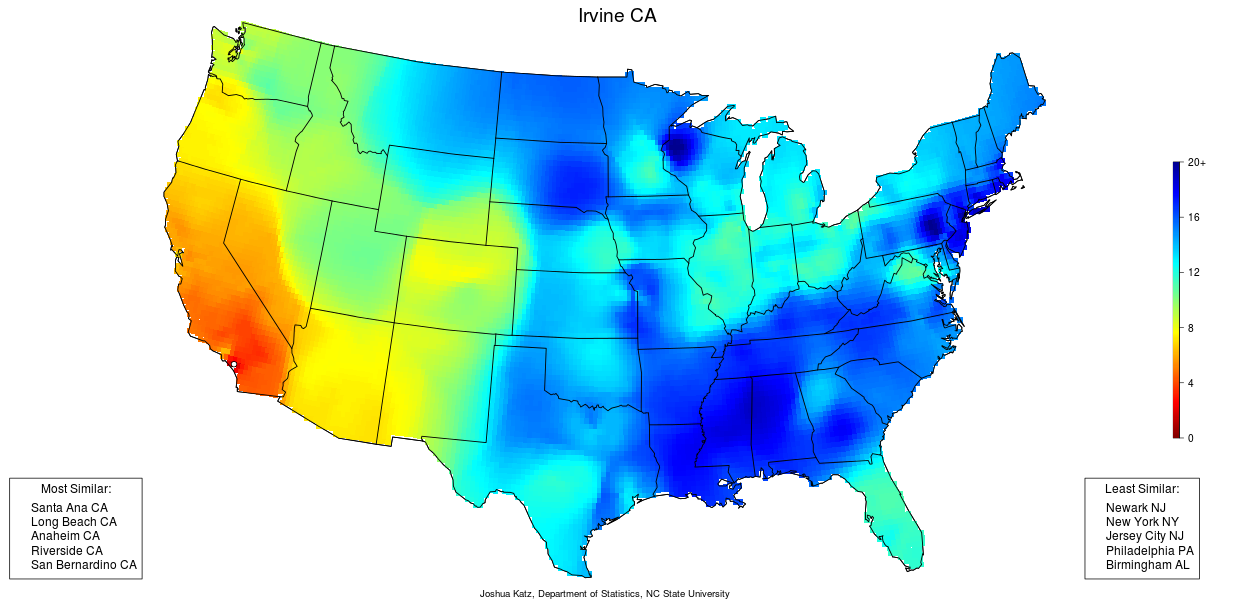
\includegraphics[scale = 0.27]{./visualization/irvine.png}

% source: http://spark.rstudio.com/jkatz/DialectMap/

\end{frame}

\begin{frame}[t]\frametitle{What cities are most similar to Davenport, IA?}    
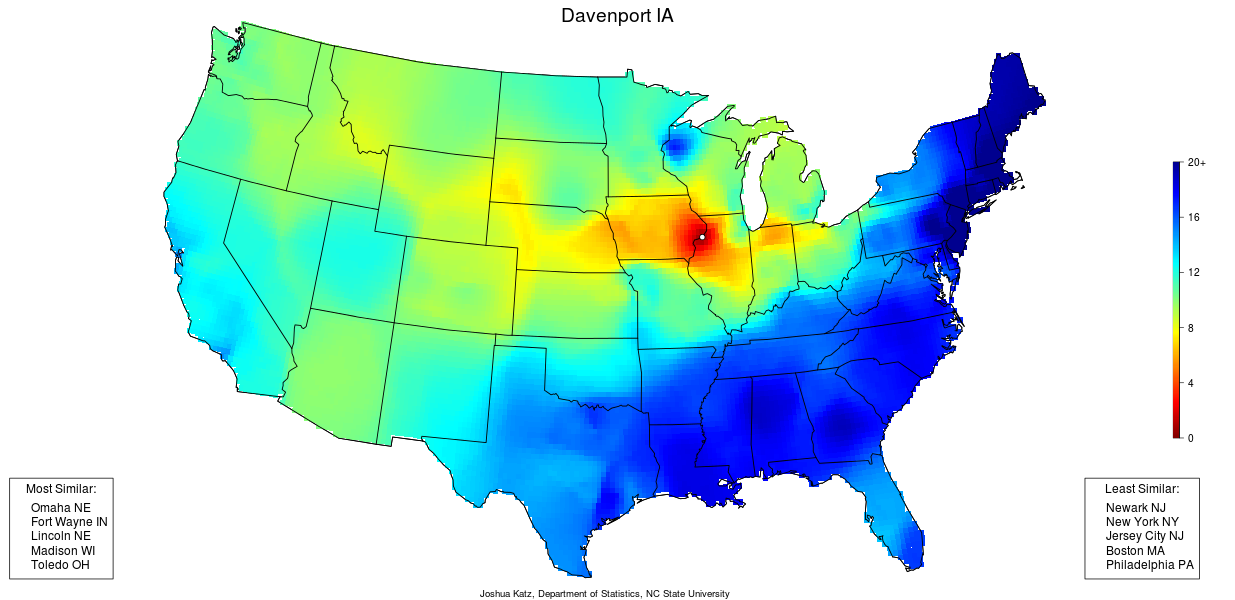
\includegraphics[scale = 0.27]{./visualization/davenport.png}
\end{frame}


% - - - - - - - - - - - - - - - - - - - - - - - - - - - - - - - -%
%						k-NN for Vernacular example
% - - - - - - - - - - - - - - - - - - - - - - - - - - - - - - - -%
\subsubsection{k-NN to predict where someone is from}

\begin{frame}[t]\frametitle{Using Vernacular to predict where someone is from}    
	Let's say you have a new person who takes the survey, how would you predict where they are from?
	
	\pause

	\begin{itemize}
		\item[]
		\item calculate $d(p_{new}, p_n)$, find $k$ people who are the most similar (have the lowest Euclidian distance ($d(p_{new}, p_n)$))
		\item Predict the region to be the majority of the $k$ peoples regions
	\end{itemize}
	\vspace{5 mm}

	\pause
	This is called {\bf{k-Nearest Neighbors}} algorithm!
\end{frame}

\begin{frame}[t]{Where else do they use k-NN algorithm?}
Amazon.com\\
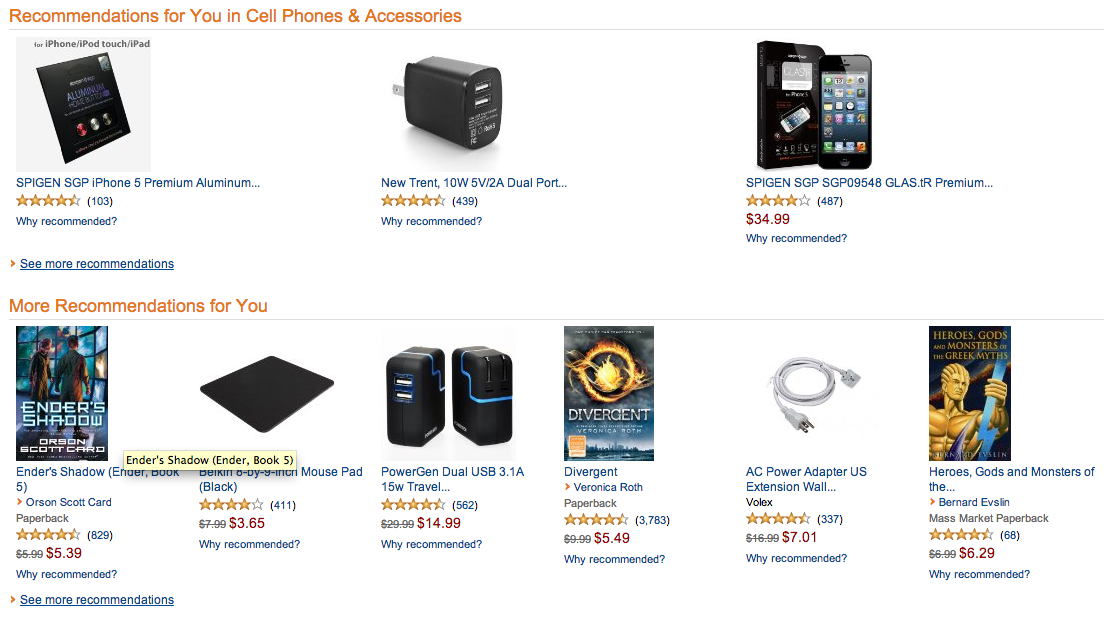
\includegraphics[scale = 0.27]{./visualization/amazon.png}
\end{frame}

\begin{frame}[t]{Where else do they use k-NN algorithm?}
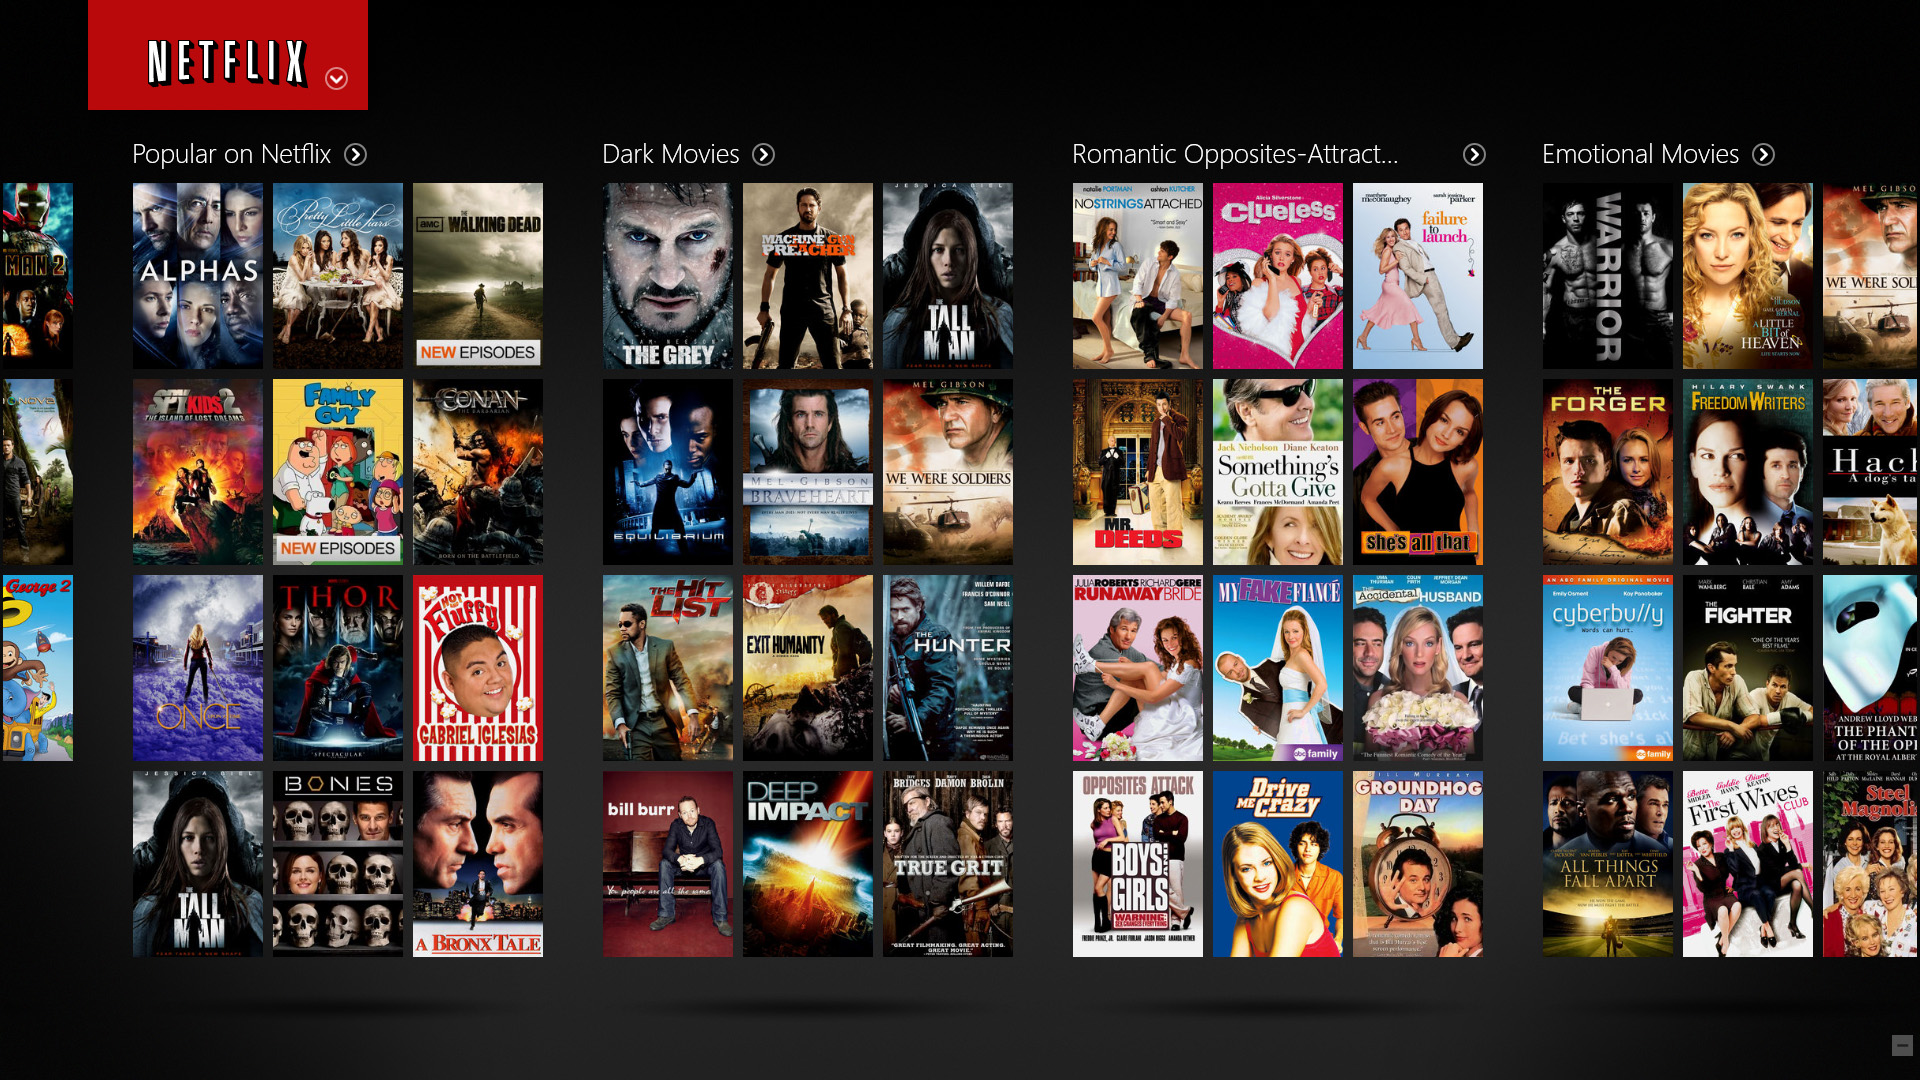
\includegraphics[scale = 0.17]{./visualization/netflix.jpg}
\end{frame}

\begin{frame}[t]{Where else do they use k-NN algorithm?}
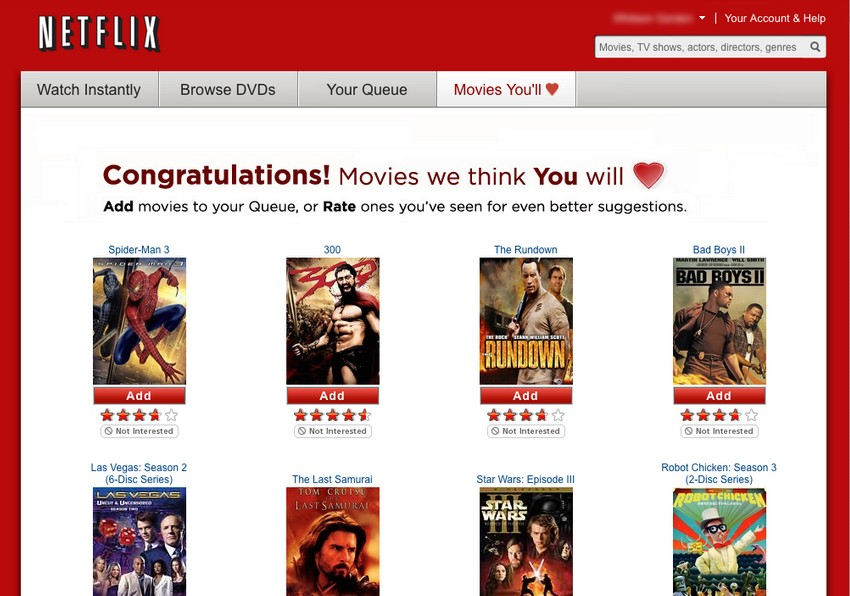
\includegraphics[scale = 0.45]{./visualization/netflix2.jpg}
\end{frame}


\begin{frame}[t]{Vernacular example - What did we learn?}
\begin{itemize}
	\item Responses to questions on Vernacular give us some interesting insights into the regions of the U.S.
	\item We can get a measure of similarity in vernacular using people's responses to the survey
	\item We can use this to predict where a new person is from! (k-NN)
	\item[]
	\item This is one of my favorite examples because it's:
	\begin{itemize}
		\item[1.] Fun to learn about this stuff
		\item[2.] It shows us improvement from iteration.
	\end{itemize}
\end{itemize}
\end{frame}

\begin{frame}[t]\frametitle{Let's go back to the `soda' example}
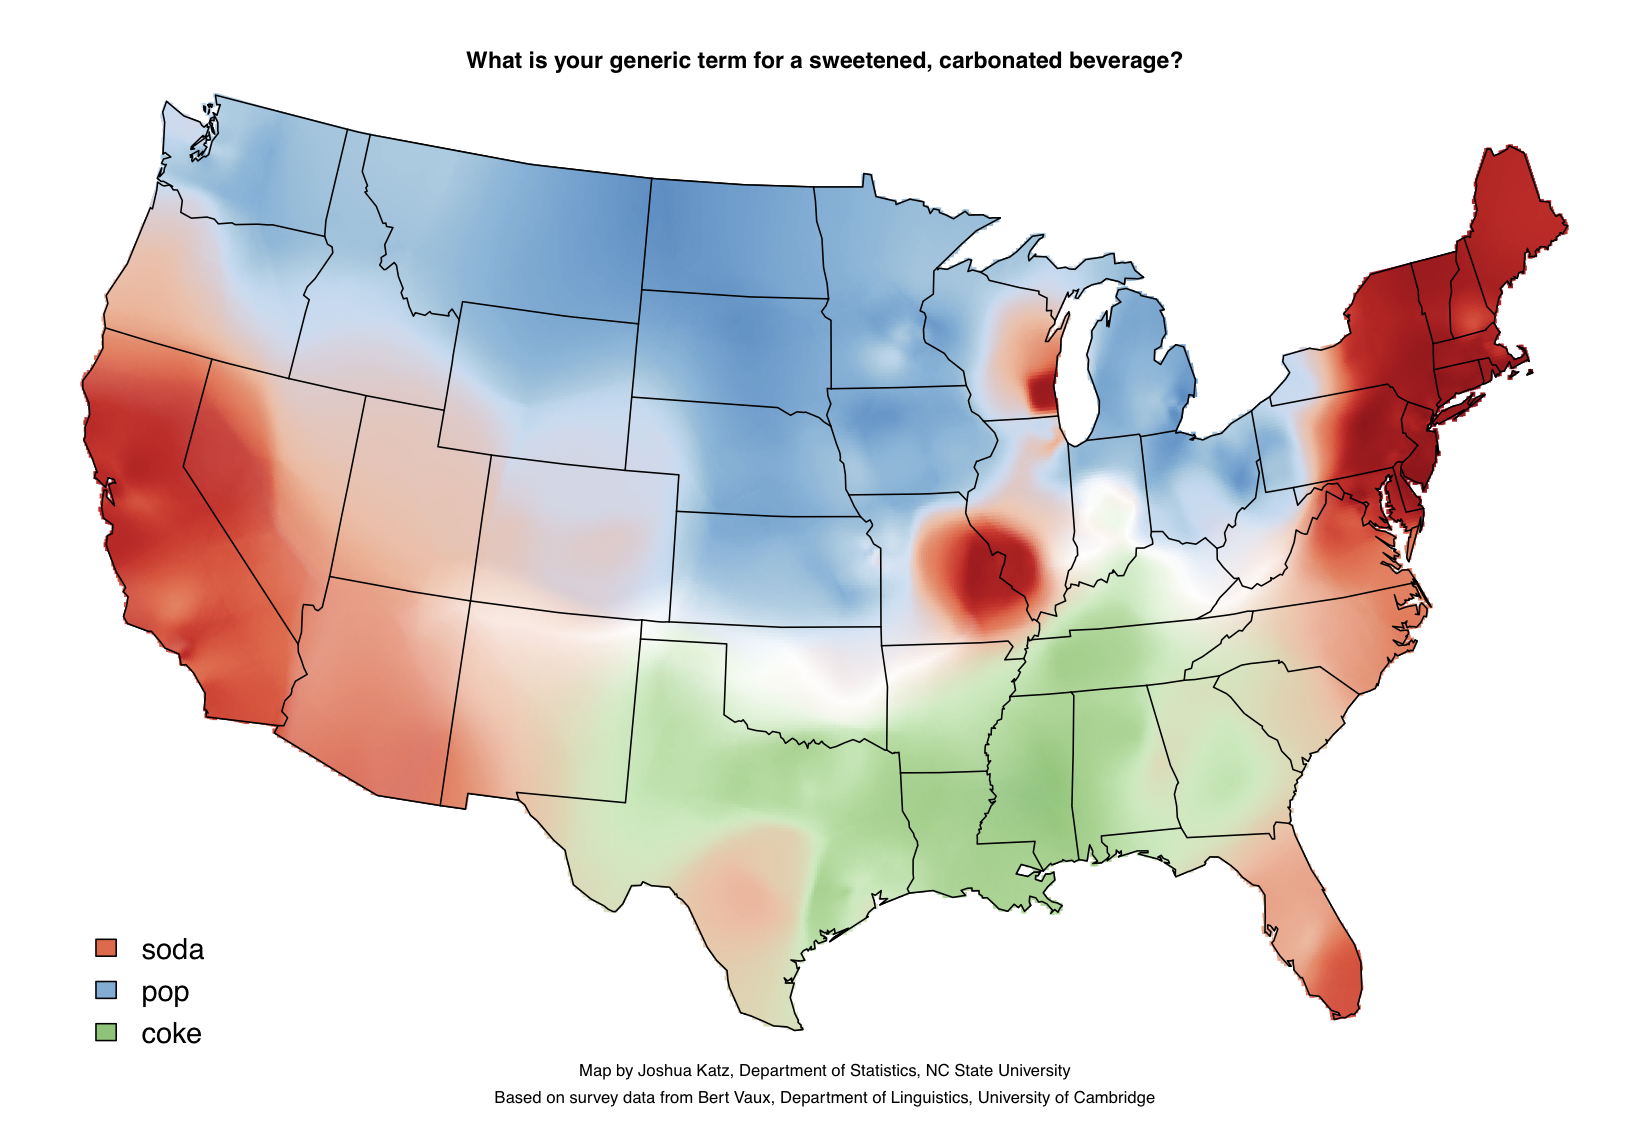
\includegraphics[scale = 0.4]{./visualization/sodapopcoke.png}
\end{frame}

\begin{frame}[t]\frametitle{Let's go back to the `soda' example}
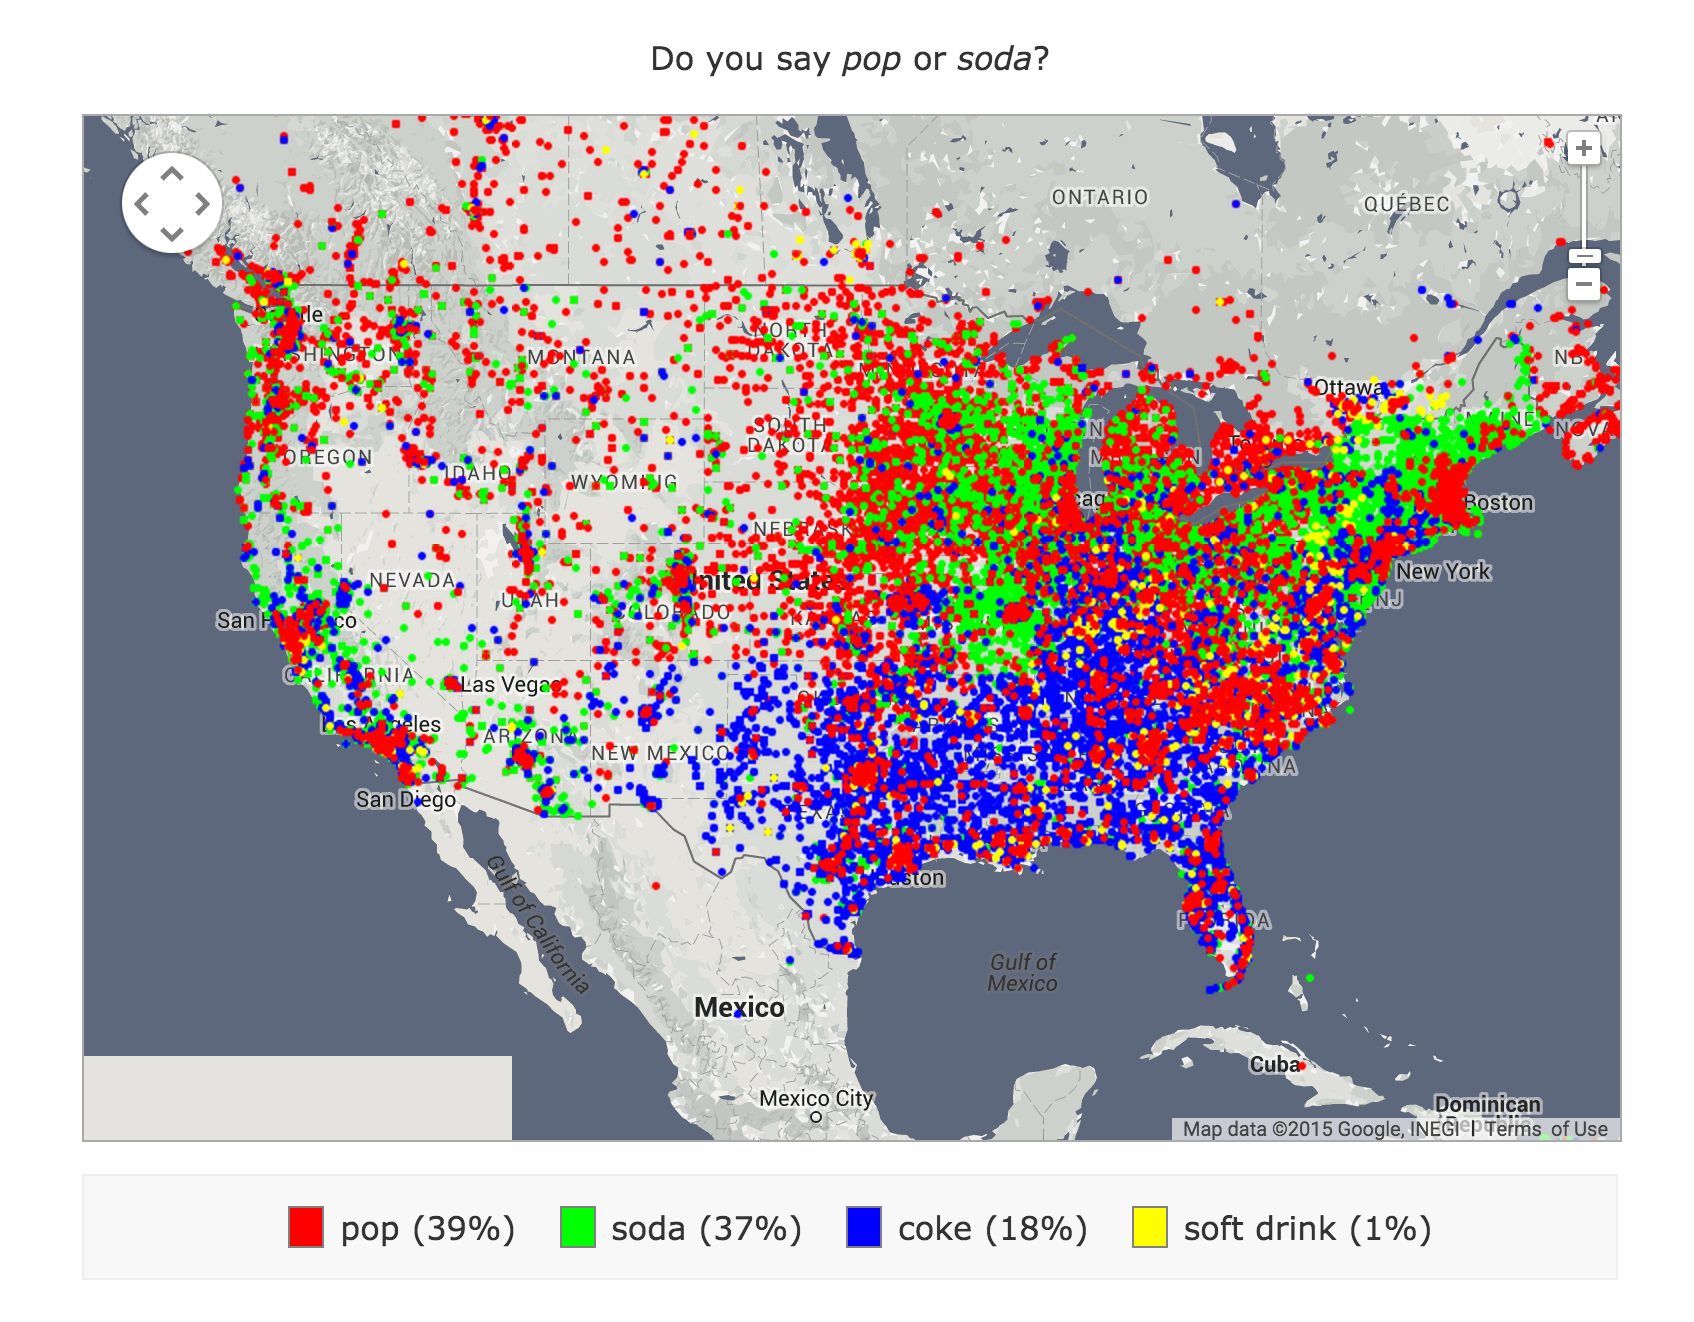
\includegraphics[scale = 0.35]{./visualization/sodapopcoke_original.png}
\end{frame}




% % % % % % % % % % % % % % % % % % % % % % % 
\comment{
% % % % % % % % % % % % % % % % % % % % % % % 

		% - - - - - - - - - - - - - - - - - - - - - - - - - - - - - - - -%
		%						Animating Wind Data
		% - - - - - - - - - - - - - - - - - - - - - - - - - - - - - - - -%

		\subsection{Visualizing Data - animation}

		\begin{frame}[t]\frametitle{Visualizing Hurricane Sandy}
		\begin{center}
		{\large{October 30, 2012}}	
		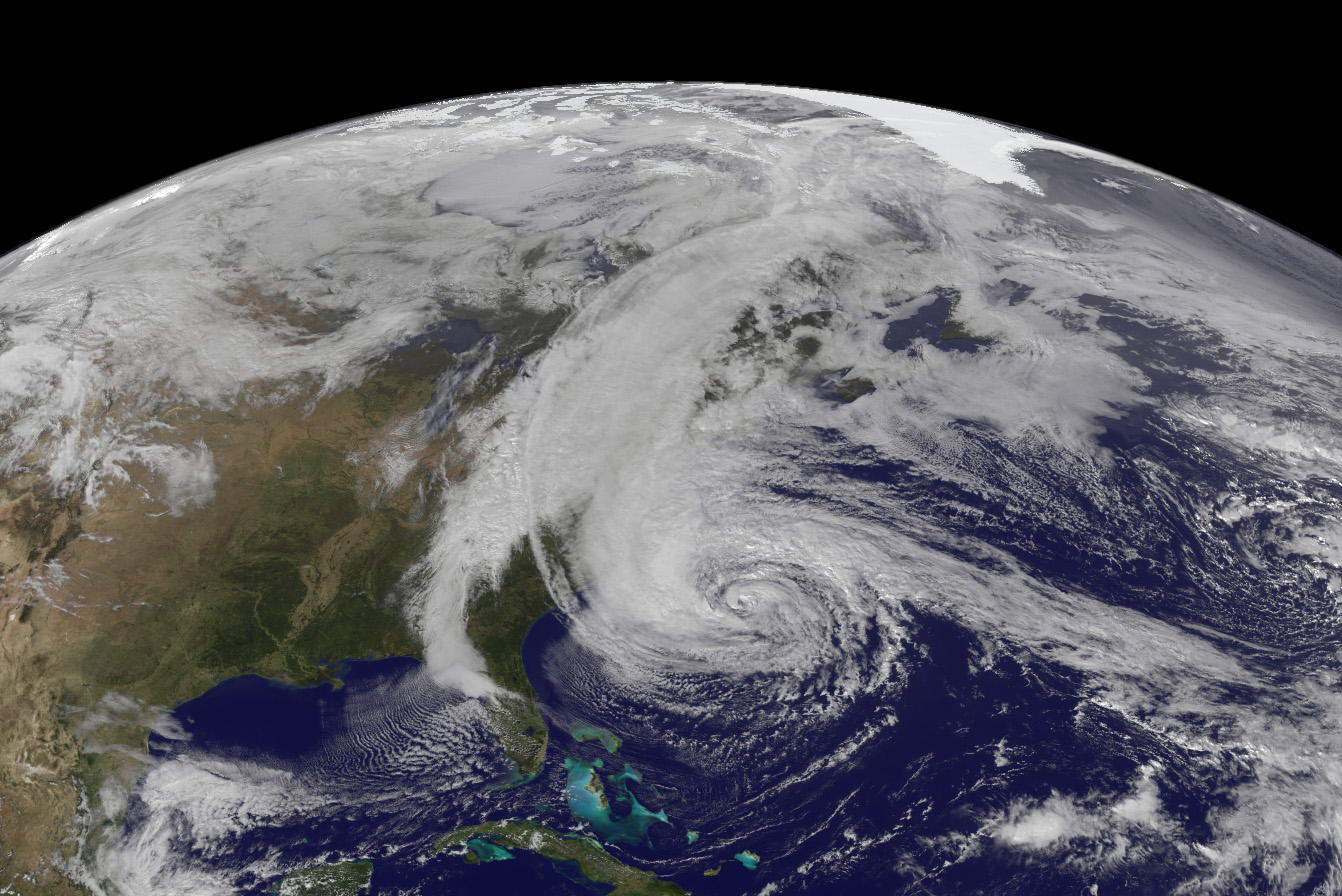
\includegraphics[scale = 0.23]{./visualization/sandy1.jpg}
		\end{center}
		\end{frame}

		\begin{frame}[t]\frametitle{Visualizing Hurricane Sandy}
		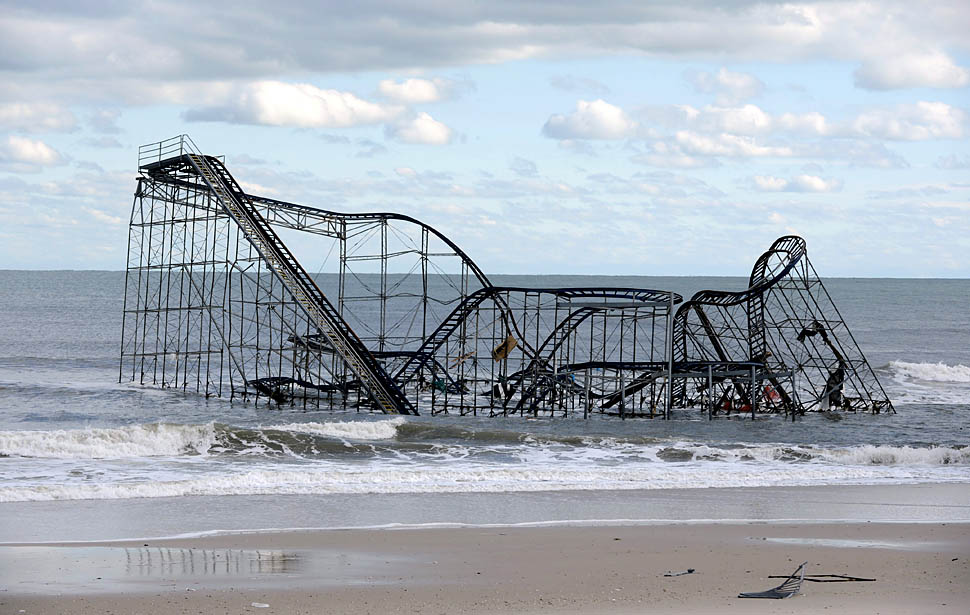
\includegraphics[scale = 0.3]{./visualization/sandy2.jpg}
		\end{frame}

		\begin{frame}[t]\frametitle{Visualizing Hurricane Sandy}
		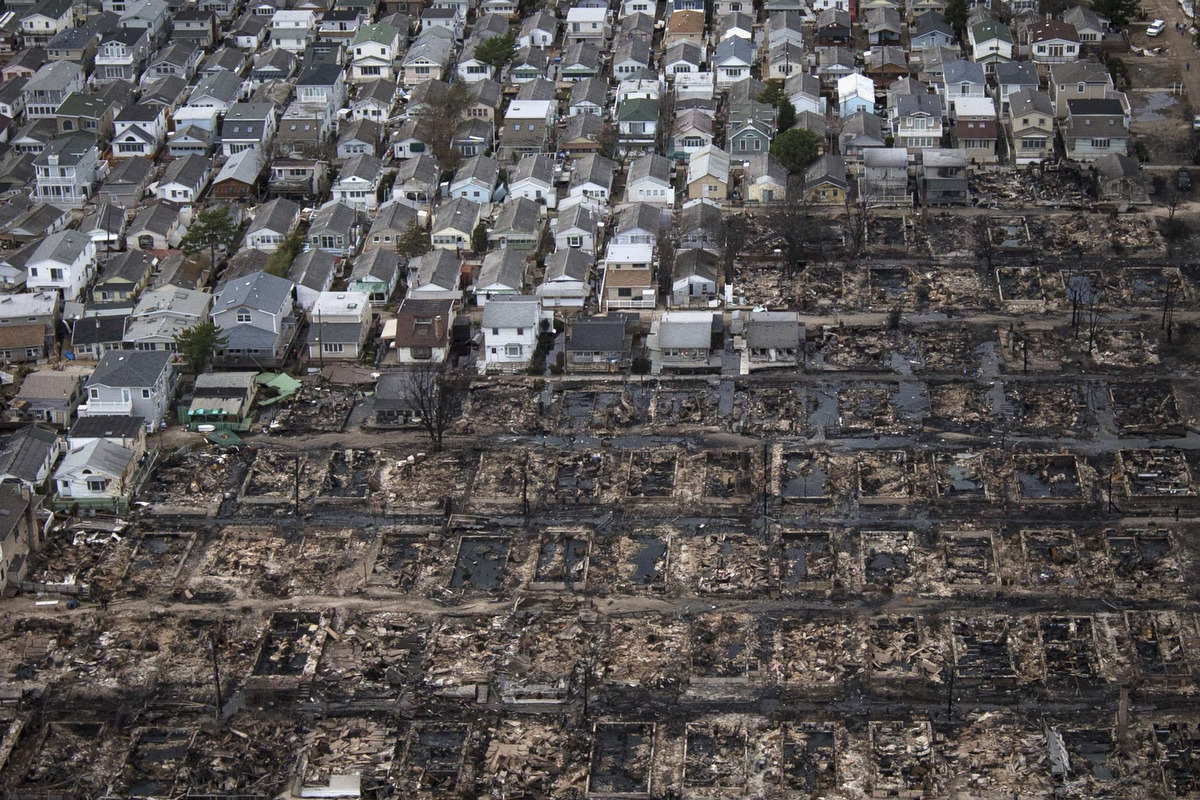
\includegraphics[scale = 0.7]{./visualization/sandy3.jpg}
		\end{frame}


		\begin{frame}[t]\frametitle{Wind Data and animation}
			The National Oceanic and Atmospheric Administration (NOAA) releases hourly information on wind data, the release looks something like this:\\
			\pause
			\begin{center}
			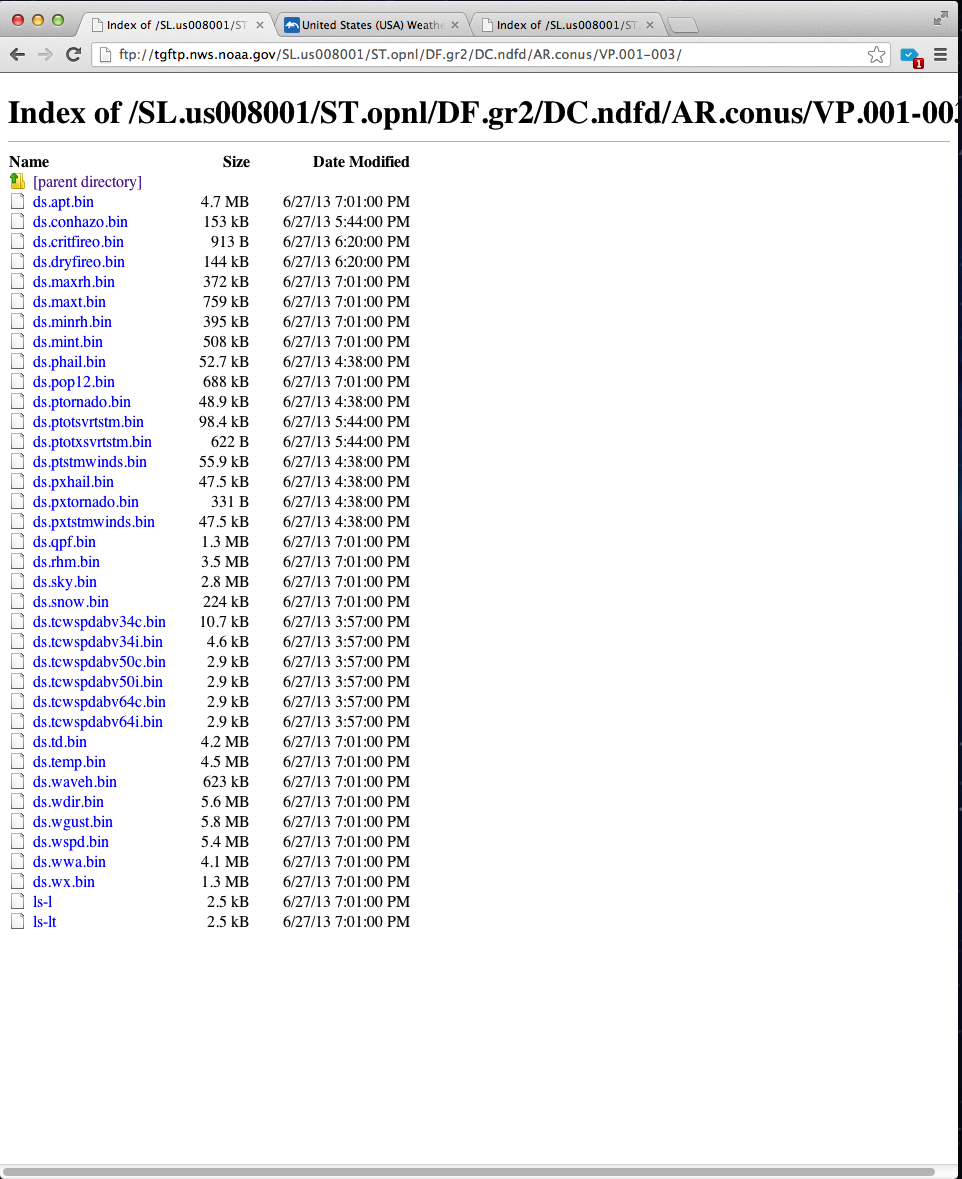
\includegraphics[scale = 0.15]{./visualization/windData_db.png}\\
			\end{center}
		\end{frame}

		\begin{frame}[t]\frametitle{Wind Data and animation}
		But in 2012 Fernanda Viégas and Martin Wattenberg decided that that wasn't a good enough way to make this information public, so they made these:\\
		\href{http://hint.fm/wind/gallery/oct-29.js.html}{\beamergotobutton{Hurricane Sandy - landfall: October 29, 2012}}
		\href{http://hint.fm/wind/gallery/oct-30.js.html}{\beamergotobutton{Hurricane Sandy: October 30, 2012}}\\
		Their website {\bf{hint.fm}} has many more animations of data like this.
		\end{frame}


		% - - - - - - - - - - - - - - - - - - - - - - - - - - - - - - - -%
		%						Interactive Data Visualizations
		% - - - - - - - - - - - - - - - - - - - - - - - - - - - - - - - -%

		\subsection{Interactive Data Visualizations}
		\begin{frame}[t]\frametitle{Interactive Data Visualizations}
		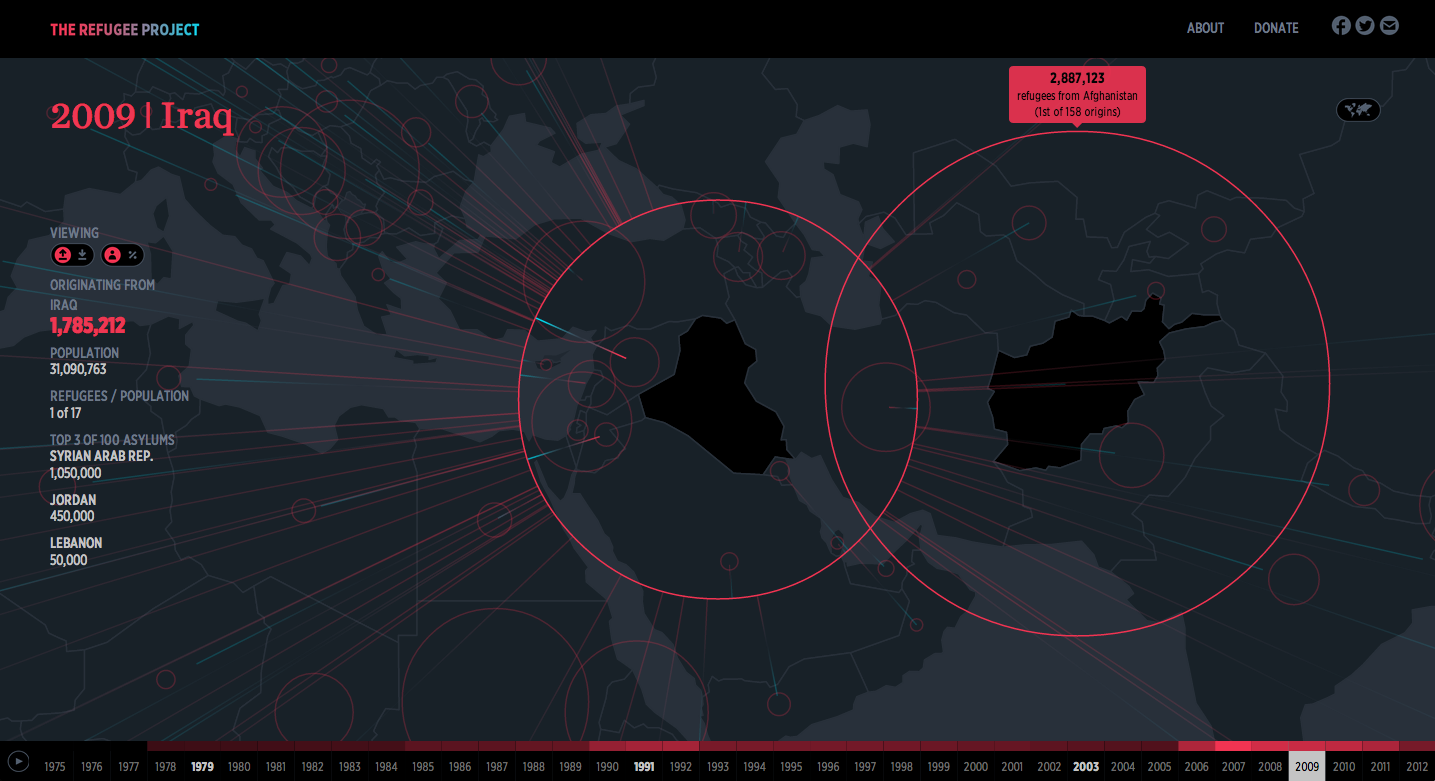
\includegraphics[scale = 0.22]{./visualization/refugee_project.png}\\
		\href{http://www.therefugeeproject.org/}{\beamergotobutton{The Refugee Project}}\\
		\end{frame}

}
% - - - - - - - - - - - - - - - - - - - - - - - - - - - - - - - -%
%						Interactive Data Visualizations
% - - - - - - - - - - - - - - - - - - - - - - - - - - - - - - - -%

\subsection{Interactive Data Visualizations}
\begin{frame}[t]\frametitle{Interactive Data Visualizations}
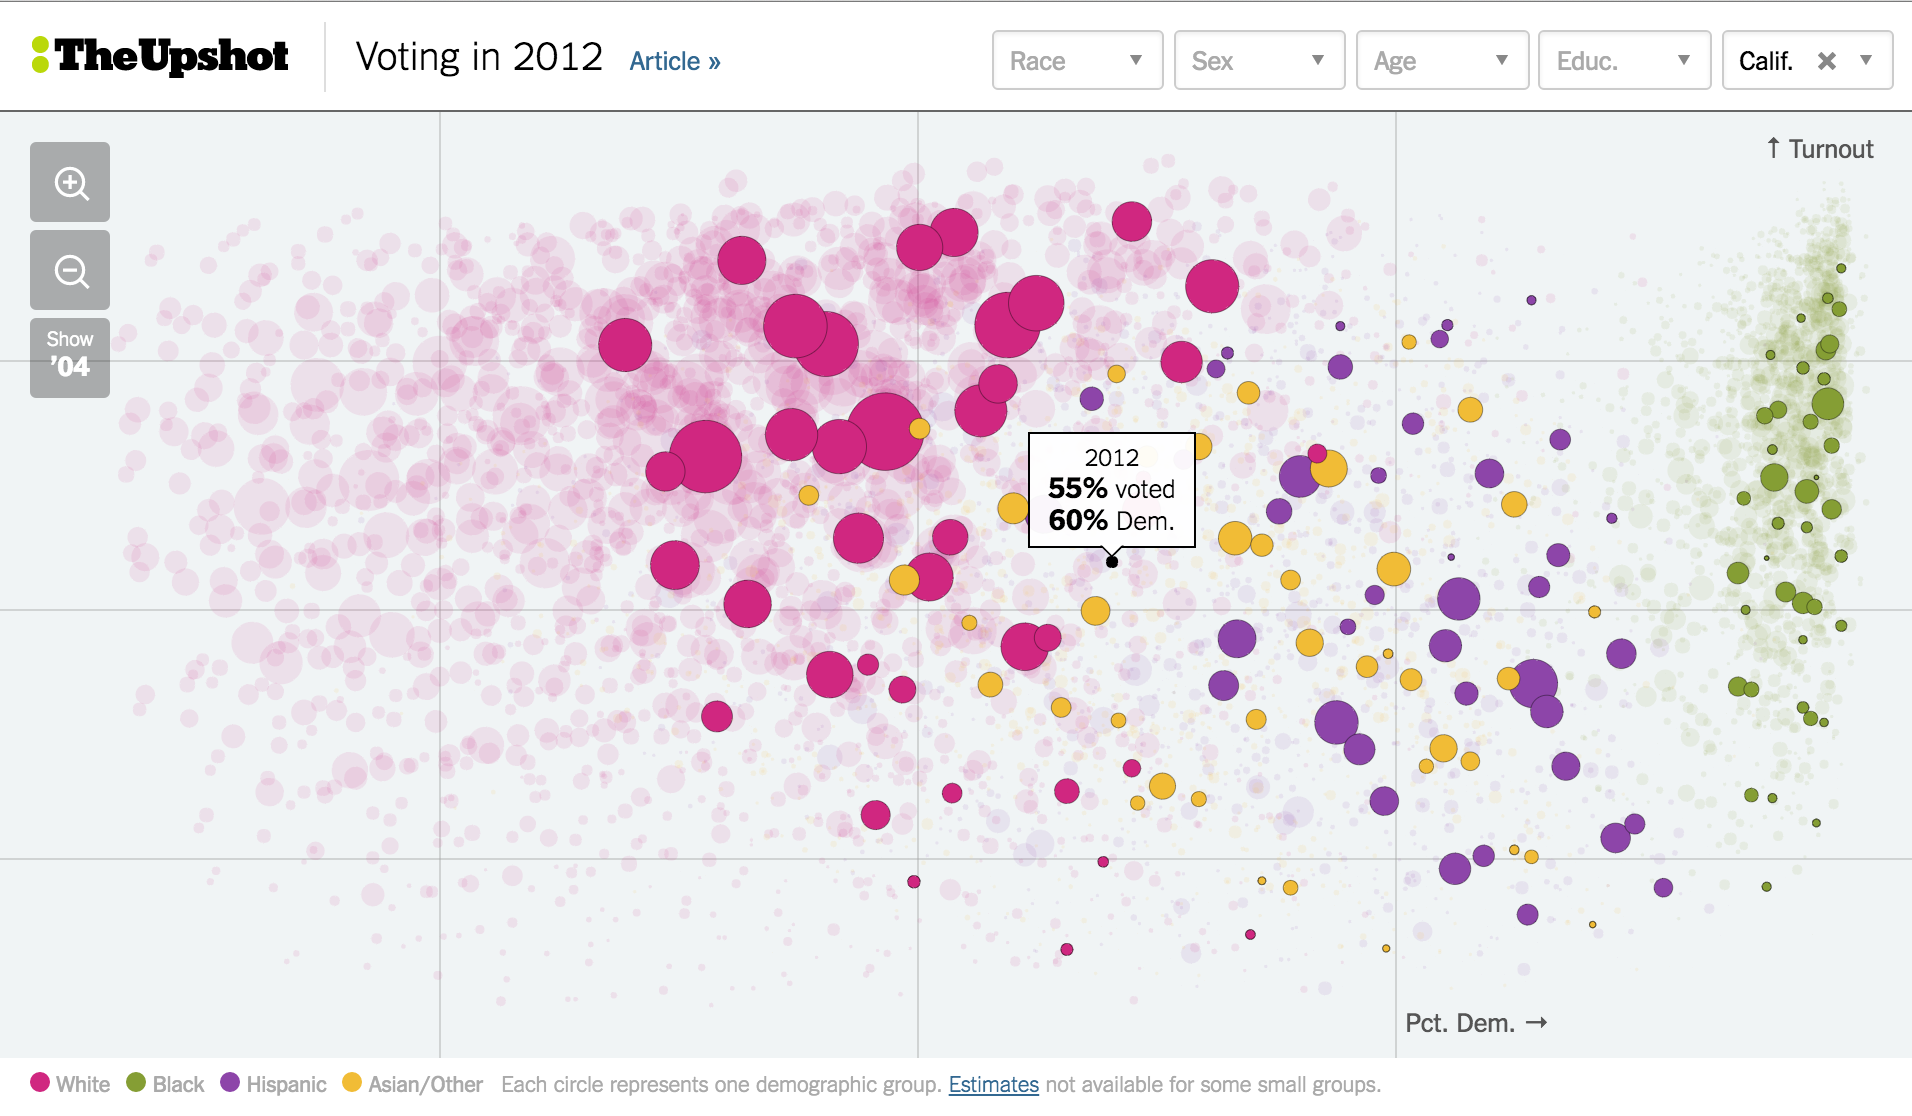
\includegraphics[scale = 0.33]{./visualization/voting_habits_viz.png}\\
\href{http://www.nytimes.com/interactive/2016/06/10/upshot/voting-habits-turnout-partisanship.html}
{\beamergotobutton{The Voting Habits of Americans Like You}}\\	
\end{frame}














% - - - - - - - - - - - - - - - - - - - - - - - - - - - - - - - -%
\begin{frame}[t]\frametitle{Conclusions: Animation and Data Visualization}
{\large{We've seen a few examples of visualizations and animations that help convey complex ideas}}
\begin{itemize}
	\item[]
	\item Facebook connection data contains tons of information
	\item[]
\pause
	\item Some basic reasoning can give us powerful tools (like k-NN)
	\item[]
\pause
	\item Animations and interactive visualizations allow people to explore and learn
	\item[]
\end{itemize}
\pause
{\bf{\Large{Thank you!}}}
\end{frame}







%%%%%%%%%%%%%%%%%%%%%%
%%%%%%%%%%%%%%%%%%%%%%
\comment{
%%%%%%%%%%%%%%%%%%%%%%
%%%%%%%%%%%%%%%%%%%%%%

	% - - - - - - - - - - - - - - - - - - - - - - - - - - - - - - - -%
	%						Monty Hall Problem
	% - - - - - - - - - - - - - - - - - - - - - - - - - - - - - - - -%
	% - - - - - - - - - - - - - - - - - - - - - - - - - - - - - - - -%

		\section[Monty Hall problem]{Monty Hall problem}

		\begin{frame}[t]\frametitle{Monty Hall - problem}
		\begin{itemize}
			\item You're on a game show where you have 3 doors (1, 2, 3) to choose from
			\item[]
			\item Behind one is a car, behind the others are goats
			\item[]
			\item You get a choice of doors, let's say you pick door 1
			\item[]
			\item The host, knowing what prize is behind what door, reveals either door 2 or 3. Whichever contains a goat. Let's say door 2
			\item[]
			\item Now the host asks "Would you like to switch to door 3?"
			\item[]
			\item Do you switch or stay? Why?
		\end{itemize}

		\end{frame}


		\begin{frame}[t]\frametitle{Monty Hall - problem}    
		\includegraphics[scale = 0.5, page = 1]{./visualization/montyHall.pdf}
		\end{frame}

		\begin{frame}[t]\frametitle{Monty Hall - problem}    
		\includegraphics[scale = 0.5, page = 2]{./visualization/montyHall.pdf}
		\end{frame}

		\begin{frame}[t]\frametitle{Monty Hall - problem}    
		\includegraphics[scale = 0.5, page = 3]{./visualization/montyHall.pdf}
		\end{frame}

		\begin{frame}[t]\frametitle{Monty Hall - problem}    
		\includegraphics[scale = 0.5, page = 4]{./visualization/montyHall.pdf}
		\end{frame}

		\begin{frame}[t]\frametitle{Monty Hall - problem}    
		\includegraphics[scale = 0.5, page = 5]{./visualization/montyHall.pdf}
		\end{frame}

		\begin{frame}[t]\frametitle{Monty Hall - problem}    
		\includegraphics[scale = 0.25, page = 6]{./visualization/montyHall.pdf}\\
		\includegraphics[scale = 0.25, page = 7]{./visualization/montyHall.pdf}\\
		\includegraphics[scale = 0.25, page = 8]{./visualization/montyHall.pdf}
		\end{frame}

		\begin{frame}[t]\frametitle{Monty Hall - problem}    
		Solution: if you switch after the door is revealed you will win 2/3 of the time. If you stay you will win only 1/3 of the time.\\
		\vspace{10 mm}
		The moral of the story can be, probability can be counter-intuitive.
		\end{frame}



%%%%%%%%%%%%%%%%%%%%%%%%%%%%%%%%%%%%%%%%%%%%%%%%%%
%%comment%%%%%%%%%%%%%%%%%%%%%%%%%%%%%%%%%%%%%%%%%
 }
%%%%%%%%%%%%%%%%%%%%%%%%%%%%%%%%%%%%%%%%%%%%%%%%%%
%%%%%%%%%%%%%%%%%%%%%%%%%%%%%%%%%%%%%%%%%%%%%%%%%%



%%%%%%%%%%%%%%%%%%%%%%%%%%%%%%%%%%%%%%%%%%%%%%
%%%%%%%%%%%%%%%%%%%%%%%%%%%%%%%%%%%%%%%%%%%%%
\end{document}
%%%%%%%%%%%%%%%%%%%%%%%%%%%%%%%%%%%%%%%%%%%%%%
%%%%%%%%%%%%%%%%%%%%%%%%%%%%%%%%%%%%%%%%%%%%%



